% !TEX encoding = UTF-8 Unicode

\documentclass[12pt,a4j]{ltjsarticle}
\usepackage{graphicx}
\usepackage{kougai}
\usepackage{enumitem}
\usepackage{amsmath}

\begin{document}

\begin{titlepage}
  \begin{center}
  
    \vspace*{20truept}
    
    {\LARGE 2022年度 卒業論文} 
    
    \vspace*{75truept}
    
    {\Huge 待ち行列問題シミュレータ教材の開発} %論文タイトル

    \vspace{10truept}

    {\Huge } %論文タイトル 長い場合 改行1

    \vspace{10truept}

    {\Huge } %論文タイトル 改行2

    \vspace{85truept}
    
    {\LARGE 指導教員 須田 宇宙 准教授}
    
    \vspace{60truept}
    
    {\LARGE 千葉工業大学 情報ネットワーク学科}
    
    \vspace{15truept}
    
    {\LARGE 須田研究室}
    
    \vspace{70truept}
    
    {\LARGE 1932008 氏名 伊豆原 嵩章 } % 氏名は消さない 学生番号 氏名 名前

    \vspace{70truept}
    
  \end{center}
  \begin{flushright}

    {\LARGE 提出日 2023年1月17日}
  
  \end{flushright}
\end{titlepage}

\tableofcontents
\clearpage

\pagestyle{plain}
\setcounter{page}{1}

\section{はじめに}
病院の受付,店舗や交通渋滞など我々の生活の至る所に待ち行列が存在する.
行列による問題は多岐にわたり生産コストや回転率など,店舗の経営などに大きく関わってくる.
最大限の利益を得るためにも,商品やサービスを提供するお客さんの回転率を高めることが重要である.
回転率を上げることは,お客さんの待ち時間が少なくなり,提供するサービスの向上にもつながる.
それら問題のアプローチ法としてモンテカルロ法を用いた待ち行列問題が存在し,シミュレーションを行うことでリソースを適正に算出し配備することができる.
待ち行列問題を用いることで,窓口数や作業員などに対応した客の平均的な待ち時間などを計算することができる.
そのため,店舗などではなるべくお客さんの待ち時間を減らし,客の回転率を上げるとともに無駄な設備投資を避けるべく,世の中の様々なところで応用されている.
例としてスーパーのレジの数,銀行の窓口数やコールセンターのオペレーターの人数などが挙げられる\cite{soumu}.

また数値計算の授業において実際に教科書や黒板からの情報だけでは直感的に理解することが困難である.
そしてモンテカルロ法の一種である「待ち行列問題」があるが,数式にパラメータを代入して答えを算出する問題と違い,教科書のような静的な教材のみでは理解しずらい.
実際に解こうとしても高い精度の解を出すために数万回程度の試行が必要となり手計算での確認は困難である.
そして先行研究として視覚的・直感的に理解できることを目的とした待ち行列問題シミュレータが存在するが,開発環境が古く現在は使用できないこと,アニメーションが画像を切り替えていくことによる擬似的なアニメーションであり,なめらかなアニメーションではなかった\cite{sotuken16}.

そこでアニメーションをより現実的な動きに寄せブラウザ上への移植及び改良することでより利用者の理解度の向上が見込めると考えた.
本研究では待ち行列についてアニメーションを用いたシミュレータ教材をブラウザ上で開発することを目的とする.
\clearpage

\section{乱数}
乱数とは数の出方が不規則で予測がつかず,次に何が出るか分からない数の数列である.
乱数は簡単に作ることができ,そして身の周りの生活にも多くの乱数が存在する.
ゲームの開発や宝くじの当選番号などもそのうちの1つである.
また多くのプログラミング言語に乱数を生成するメソッドや関数が用意されており,使用するのは容易である.
乱数は自然現象をシミュレーションするために用いられることが多い.
待ち行列問題もその自然現象のうちの1つである.
待ち行列問題も乱数を用いてシミュレーションできるが,この現象を再現するためには大量の乱数が必要となる.
そのため,コンピュータを用いて乱数を発生させるのが一般的である.
しかし,コンピュータは規則に従って動作しているので,完璧な乱数を作ることができないが,それに近い乱数を発生させることは可能である.
このようにコンピュータを用いて発生させた乱数のことを擬似乱数と呼ぶ.モンテカルロ法では以下に示すような3つの乱数を用いて計算を行う.

\subsection{一様乱数}
乱数のうち,出た数が図\ref{fig:一様乱数のグラフ}のような一様分布に従う乱数を一様乱数という.
図\ref{fig:一様乱数のグラフ}を見ての通り,どの値でも一定の値をとる.
つまり,ある区間において数値が同じ確率で出現する確率分布に従う乱数のことである.
一様乱数として身近なもので,サイコロがある.サイコロは1から6までの数値がすべて$\frac{1}{6}$の確率で出現する.
\vspace{10mm}
\begin{figure}[h]
\begin{center}
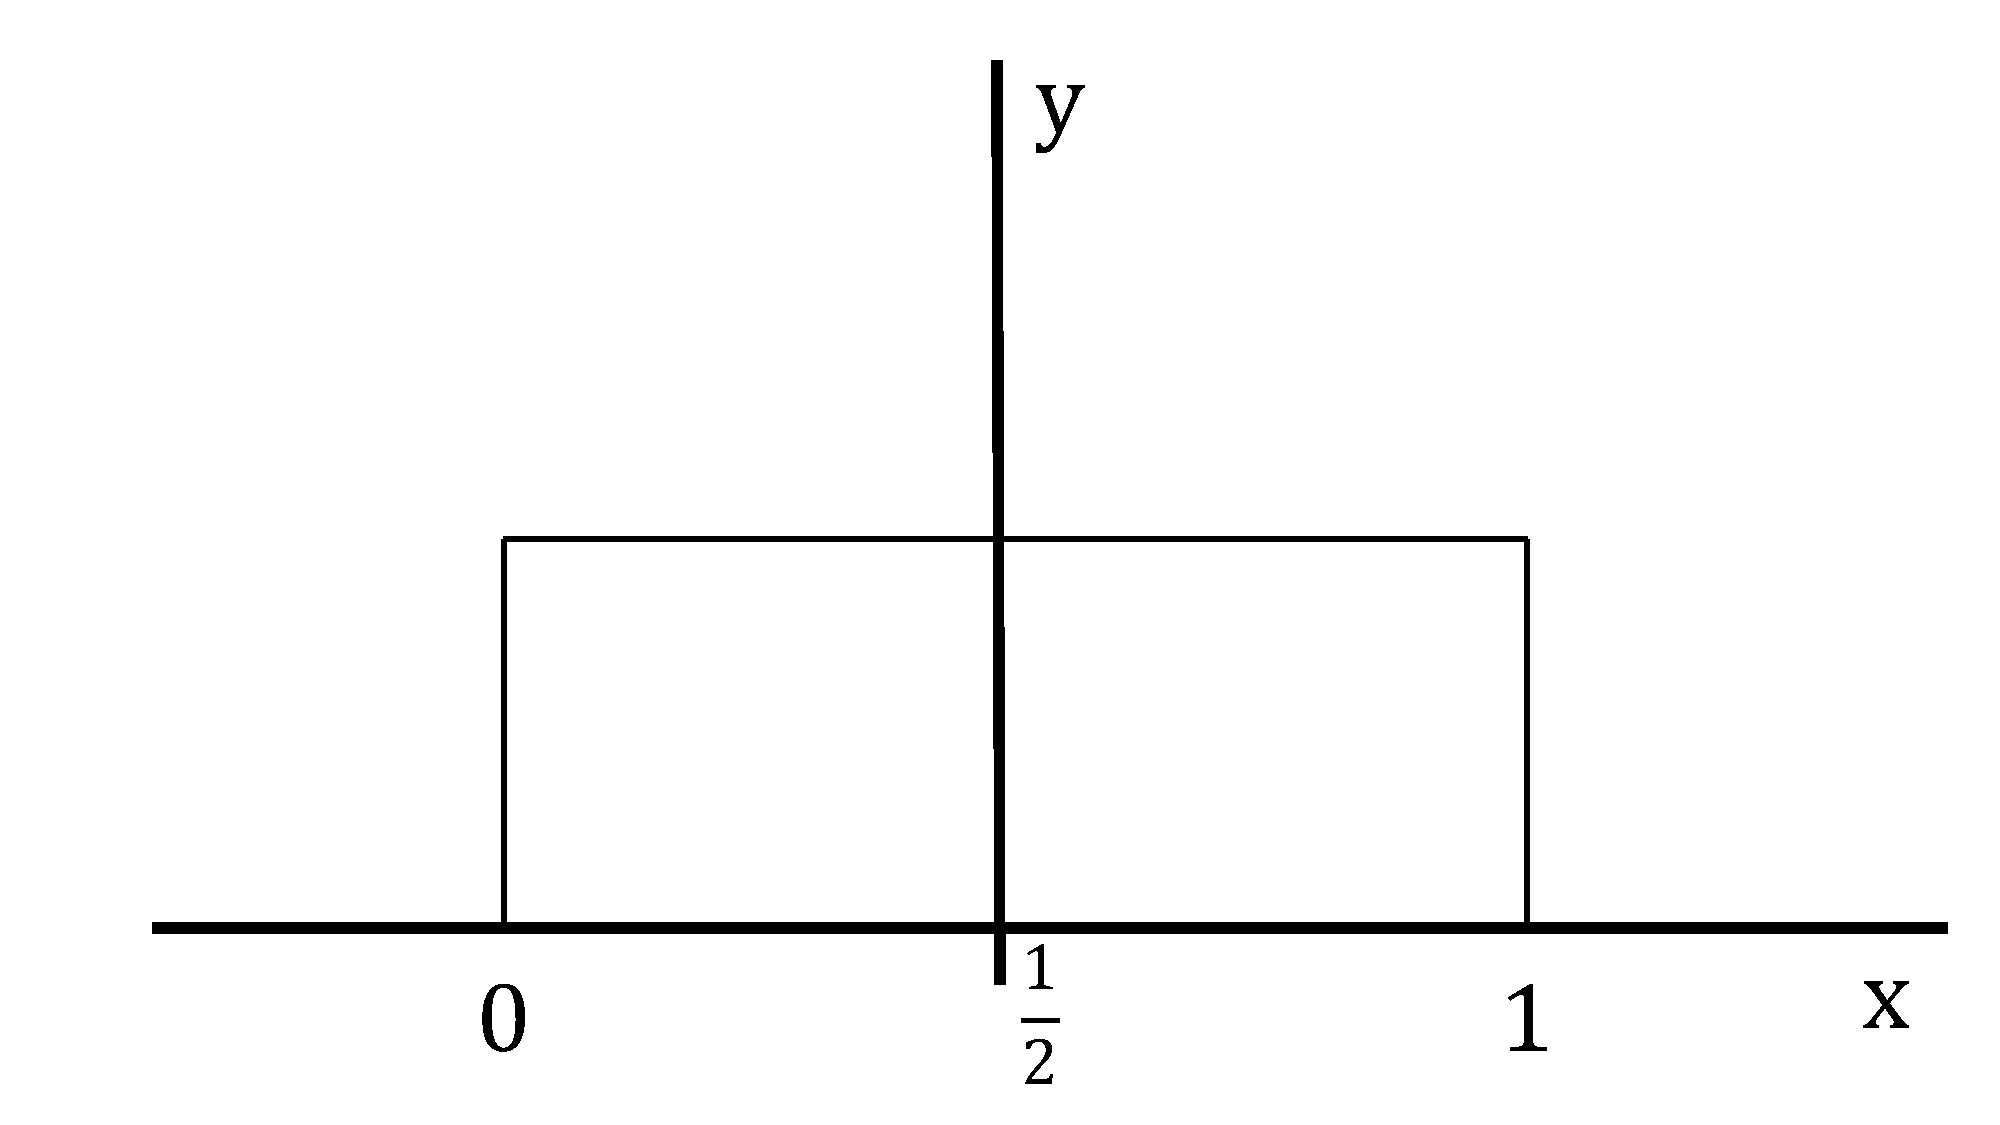
\includegraphics[width = 100mm ] {figures/itiyo.pdf}
\caption{区間(0,1)の一様乱数の確率密度関数}
\label{fig:一様乱数のグラフ}
\end{center}
\end{figure}
\clearpage

一様乱数の発生方法として,次の2通りが存在する.
1つ目はフォン・ノイマン(John Von Neumann)によって提案された平方採中法である.
図\ref{fig:平方}は,平方採中法の方法を順を追って説明している.
この方法は例えば4桁の乱数列を求める場合,図\ref{fig:平方}に示すように,まず4桁の初期整数1234を平方して,その解の中央の4桁を取り出す.
その乱数列5227を第2項とし,以下同様の方法で乱数列を求めていく方法である.
\begin{figure}[h]
\begin{center}
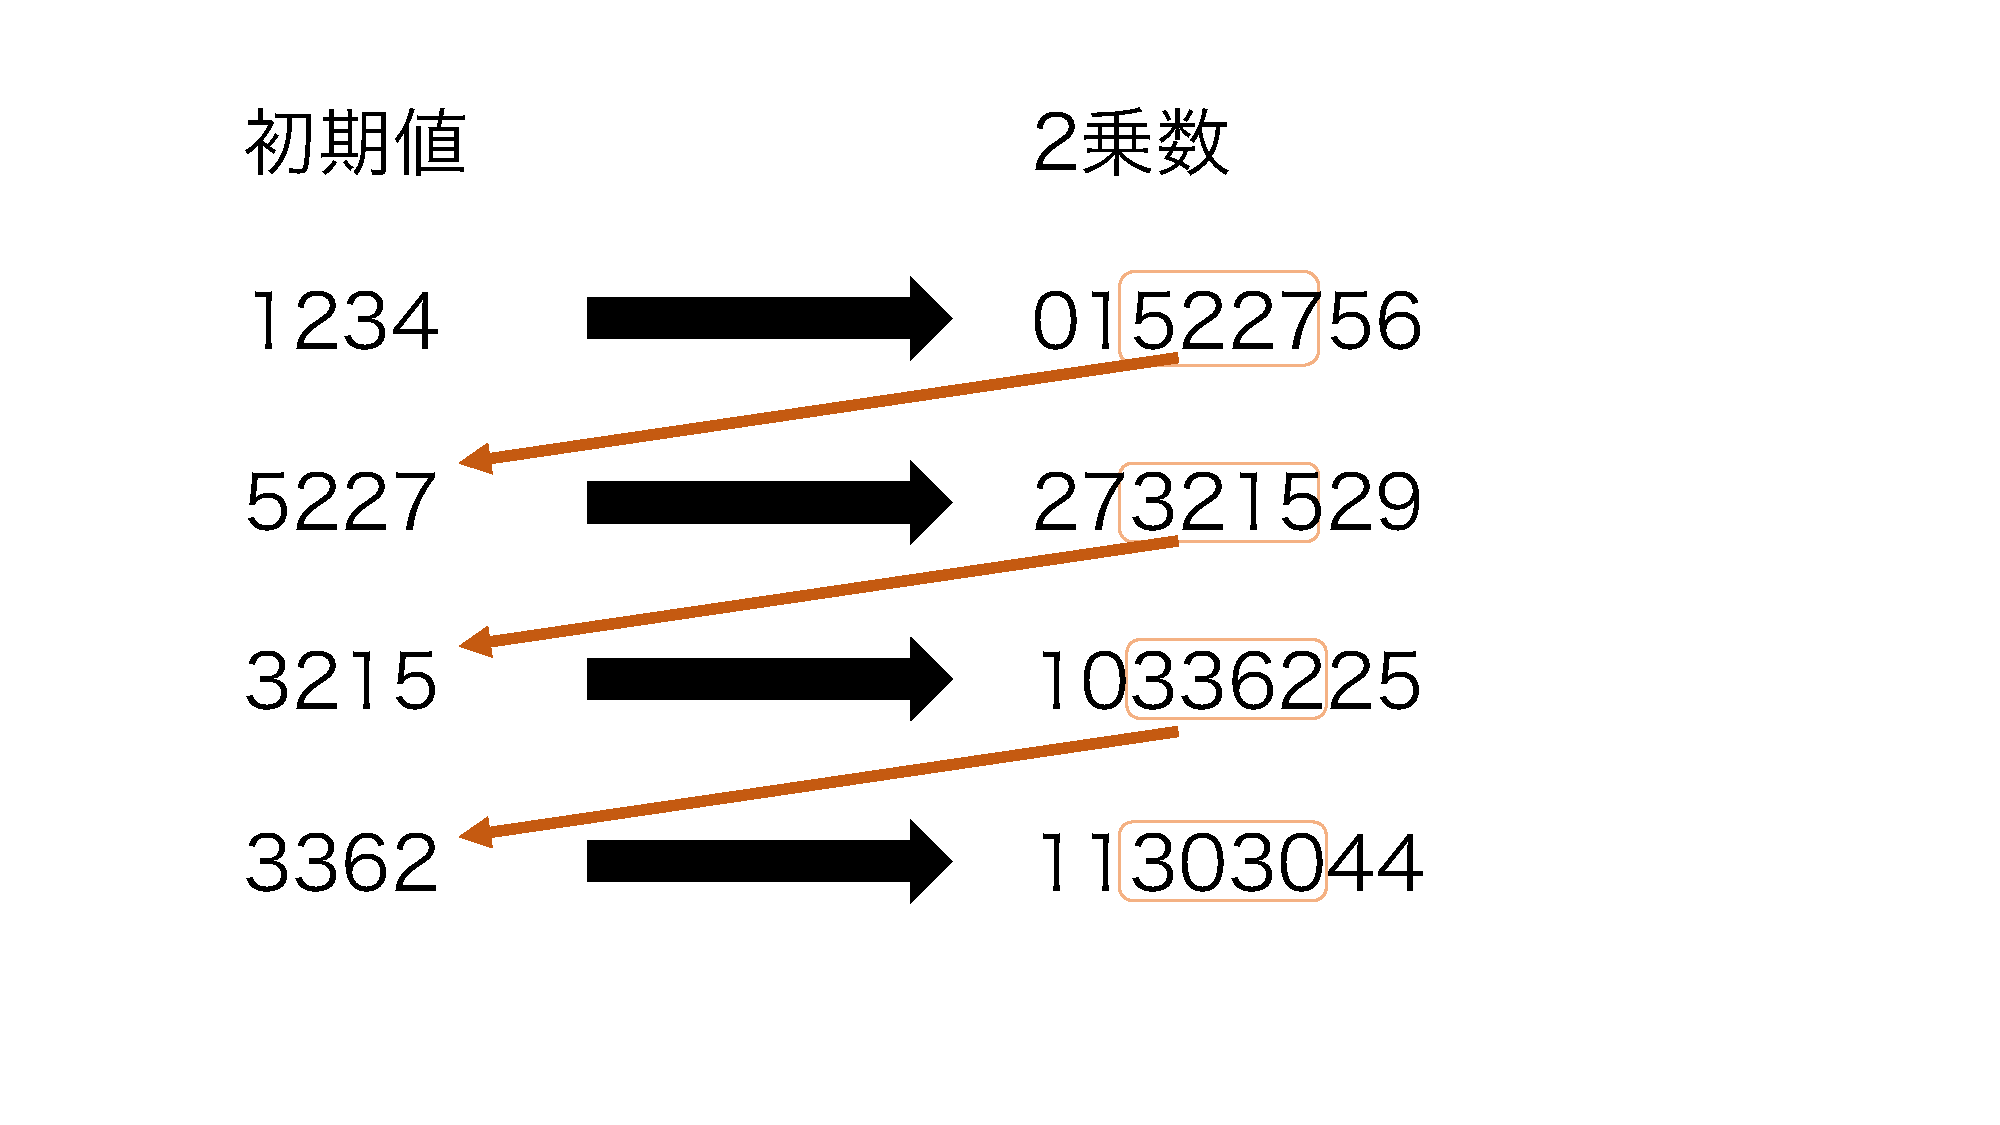
\includegraphics[width = 100mm ] {figures/heihousaisunhou.pdf}
\caption{平方採寸法による乱数生成の例} 
\label{fig:平方}
\end{center}
\end{figure}

平方採中法は計算で必要とする整数の有効桁数が求めたい整数の2倍必要になる上に,乱数列を得るための計算時間も長くなってしまう.

そこで2つ目の方法として,レーマー(H.Lehmer)により提案された乗算合同法がよくつかわれている.
乗算合同法は除算の剰余を数列化していくものである.
次式を使い,乱数を求める方法である.
\begin{enumerate}[label=(\Alph*)]
	\item  $x_{n+1} = ax_n(mod M)$
	\item $n >= 1$
\end{enumerate} 

また区間(0,1)の範囲で一様乱数を必要とする場合には,上記の方法で得られた乱数列を$M$で除算すればよい.
乗算合同法では,乱数を生成する方法として剰余を用いているので,乱数の最大値は$M$より大きくならない.
必ず$M$より小さな周期を持つことになる.
そのため$M$としては大きな値を与える必要がある.
しかし式(A)から分かるように乱数生成の計算に必要な整数の最大値($aM$)になるので,この値がコンピュータの扱える最大整数値を超えないようにする必要がある.

\clearpage

\subsection{正規乱数}
図\ref{fig:正規乱数}は正規分布の密度関数を表している.
事象として平均値を取る確率が一番大きく、平均値から離れるにつれその値を取る確率は小さくなることがグラフから読み取れる.
乱数のうち,生成の割合が図\ref{fig:正規乱数}のような正規分布に依存しているものを正規乱数という.
\vspace{8mm}
\begin{figure}[h]
\begin{center}
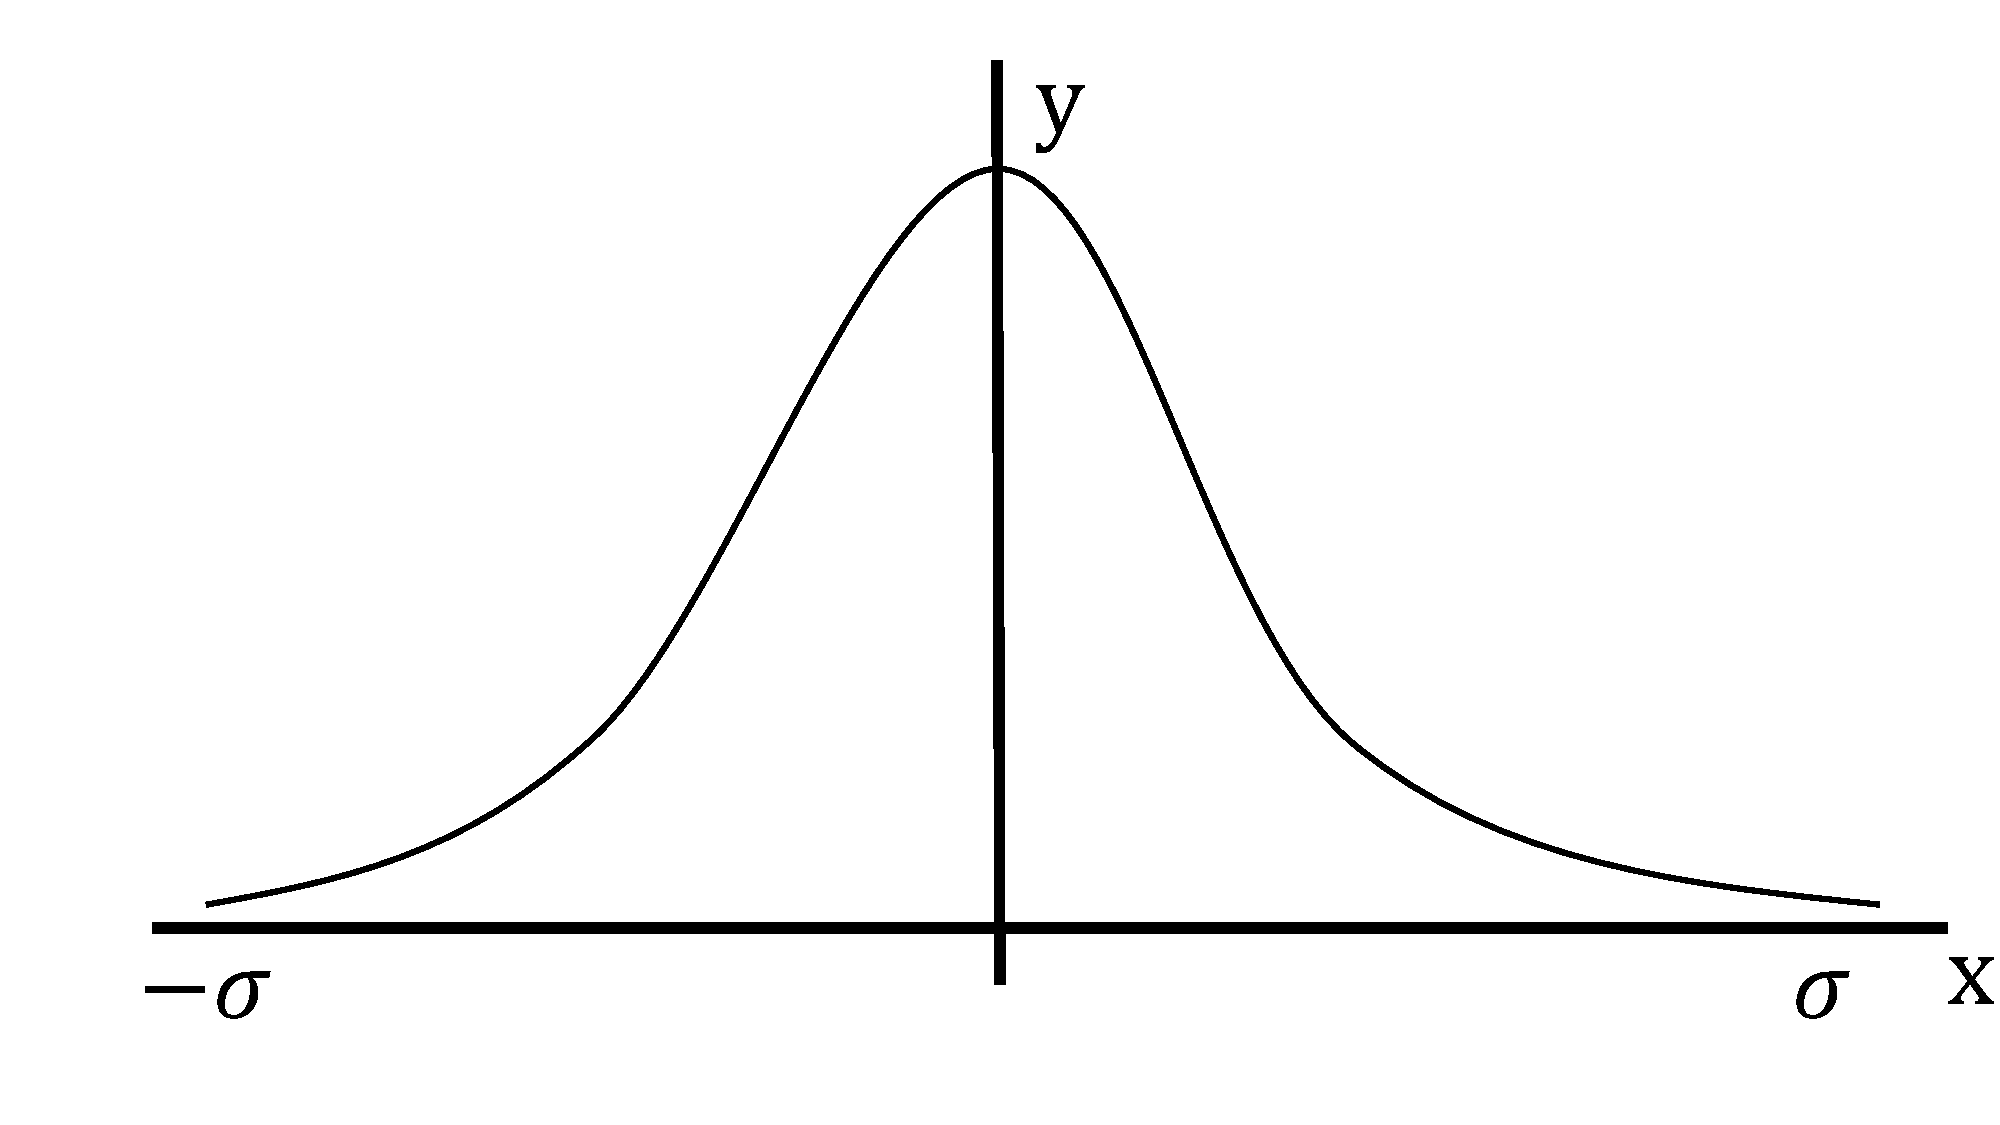
\includegraphics[width = 100mm ] {figures/seikir.pdf}
\caption{(\mu,\sigma)の正規分布の密度関数}
\label{fig:正規乱数}
\end{center}
\end{figure}

正規乱数は「ある値を中心にして,偶発的に生じる事柄は正規分布に従う」という法則に基づいて生成することができる.
また正規乱数は一様乱数から生成することができる.
区間(0,1)で一様乱数をとりだして平均し,これを繰り返して新たな乱数の集合を作る.
一様な乱数を取り出してこの平均を取るので,その値は区間の平均値($\frac{1}{2}$)を中心にばらつく.
またこのようにして生成した乱数列の分布は,平均値が$\frac{1}{2}$,標準偏差が$\frac{1}{12}$という正規分布になるという性質がある.
このことを中心極限定理と呼び,これを利用して正規乱数に極めて近い分布を持つ乱数列を生成することができる.

取り出す乱数の個数$N$はある程度大きな数字が必要であるが,$N$を12とすれば平均値も標準偏差も整数で表せられるので,一般的には$N = 12$が使われている.

取り出した乱数の総和($\nu=\gamma_1+\gamma_2+・・・+\gamma_{12}$)の集合は全て12倍されて,平均値は6,標準偏差が1になるので,これらの集合から6引いた値

\begin{enumerate}[label=(\alph*)]
	\item $\nu =  \nu=\gamma_1+\gamma_2+・・・+\gamma_{12}-6$
	
は平均値が0で,標準偏差が1の正規乱数となる.
	
よって平均値が$\mu$で,標準偏差が$\sigma$の正規乱数は
	\item $\mu+\sigma\nu$
	
という関数で表すことができる.
\end{enumerate} 

\clearpage

\subsection{指数乱数}
図\ref{fig:指数乱数のグラフ}は指数分布のグラフである.
指数乱数はランダムなイベントの発生間隔を表す分布である.
日常で使用されている例として「地震が起きる間隔」や「電球の寿命」などを表す分布として使われいる\cite{Exponential}.
乱数のうち,生成の割合が図\ref{fig:指数乱数のグラフ}のような指数分布に依存する.
\vspace{5mm}
\begin{figure}[h]
\begin{center}
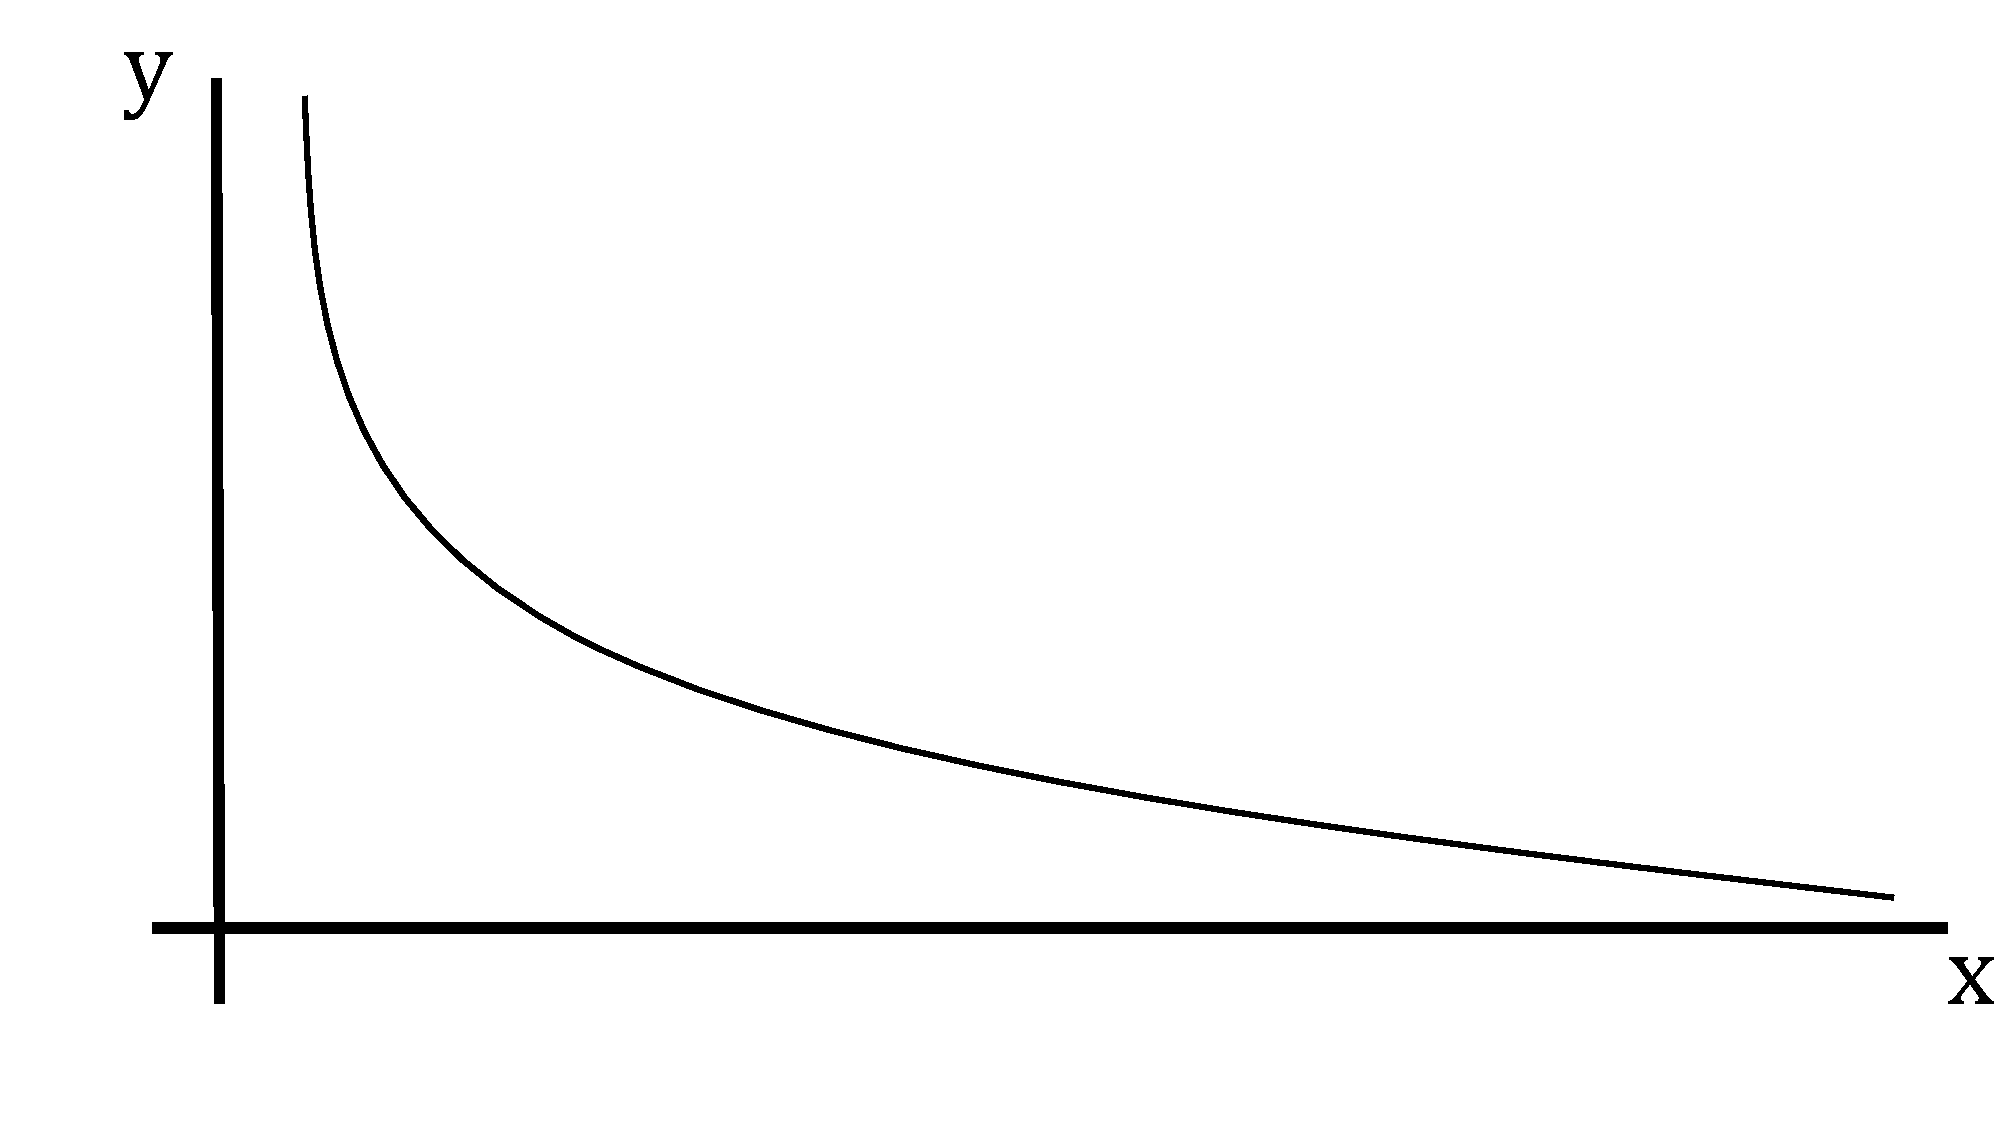
\includegraphics[width = 100mm ] {figures/sisu.pdf}
\caption{指数分布の概形}
\label{fig:指数乱数のグラフ}
\end{center}
\end{figure}

性質として「小さな値は多く生じ,大きな値はあまり起こらない」偶発的な値を発生させるということがある.
指数乱数の生成方法は,ある分布の乱数の確率分布を積分すると,一様乱数になるという性質を利用して生成する.
このような生成方法を逆変換法という.例えば$\nu$を指数乱数とし,$\gamma$を一様乱数とすると次のような関係式になる.
\begin{enumerate}[label=(\roman*)]
\item $\int_0^\gamma{\alpha}exp(-\alpha\nu)dx = \gamma$

\noindent
この式を積分して変形すると

\item $\nu = -(\frac{1}{\alpha})ln(1-\gamma)$

\noindent
が得られる.ここで$\gamma$は区間(0,1)の一様乱数なので,1-$\gamma$も一様乱数になる.よって指数乱数の生成方法は

\item $\nu = -(\frac{1}{\alpha})ln\gamma$
\end{enumerate} 
\noindent
という式に基づく.この指数分布による乱数は,ある系に偶発的に顧客が入ってくる時間間隔のモデルとしてよく用いられ,(e)式で表された客の流れを最も簡単な流れ,またはポアソン分布と呼んでいる.この場合,パラメータ$\alpha$は客の流れ密度に相当する.

\clearpage

\section{ 待ち行列問題}
\subsection{待ち行列問題}
待ち行列問題とは,$n$ 箇所の窓口が開いていてサービスに $\delta$時間かかる時の窓口で客がサービスで受けられるまでの平均待ち時間 t を計算することである.このとき($N+1$)番目の客が入ってくる時刻$t_{N+1}$は下記の式で表すことができる.\\

\begin{eqnarray}
t_{N+1}=t_N+\tau\\
t_0=0\\ 
\tau=-\frac{1}{\alpha}\ln\gamma
\end{eqnarray}
同様に,個々の客のサービス時間は以下の式で表せれる.\\ 
\begin{equation}
\delta=\delta_0+\sigma\nu
\end{equation}

(\tau:次の客が入ってくる時間間隔の期待値,\alpha:客の流れの密度,\gamma:区間(0,1)の一様乱数,\delta:客一人が受けるサービスの時間,$\delta_0$:サービスに必要な平均時間,\sigma:標準偏差,$\nu=\gamma_1+\gamma_2+・・・+\gamma_{12}-6$)
実際に待ち行列問題を解くためには以下の4つのパラメータを定め,乱数を発生させて計算していく.

\begin{enumerate}[label=(\Roman*)]
	\item 客の流れ密度$\alpha$
 	\item 窓口の数$n$
 	\item サービスに必要な平均時間$\delta_0$
 	\item サービスに必要な時間の標準偏差$\sigma$
\end{enumerate} 

\clearpage

図\ref{fig:待ち行列概要}は窓口サービスと顧客入場の関係について図で表したものである.
$t_k$は待ち行列を表しており,窓口である$n_m$が客で埋まっている時,$t_k$に格納される.
客の入場頻度は指数乱数に基づき,処理時間は正規乱数に基づいている.
$N$番目の客はどこかの窓口が空いていればその場所でサービスを受けられるが,全てが使用中だといずれかの窓口が空くまで待たされる.
この待ち時間を集積し全客数で割れば一人当たりの平均待ち時間が計算される.
しかし実際には営業時間や曜日等によって客の入ってる分布が異なるため,乱数などの偶発的な確率変数を用いて試行錯誤的に問題を解いていく数値計算法である.

\vspace{5mm}
\begin{figure}[h]
\begin{center}
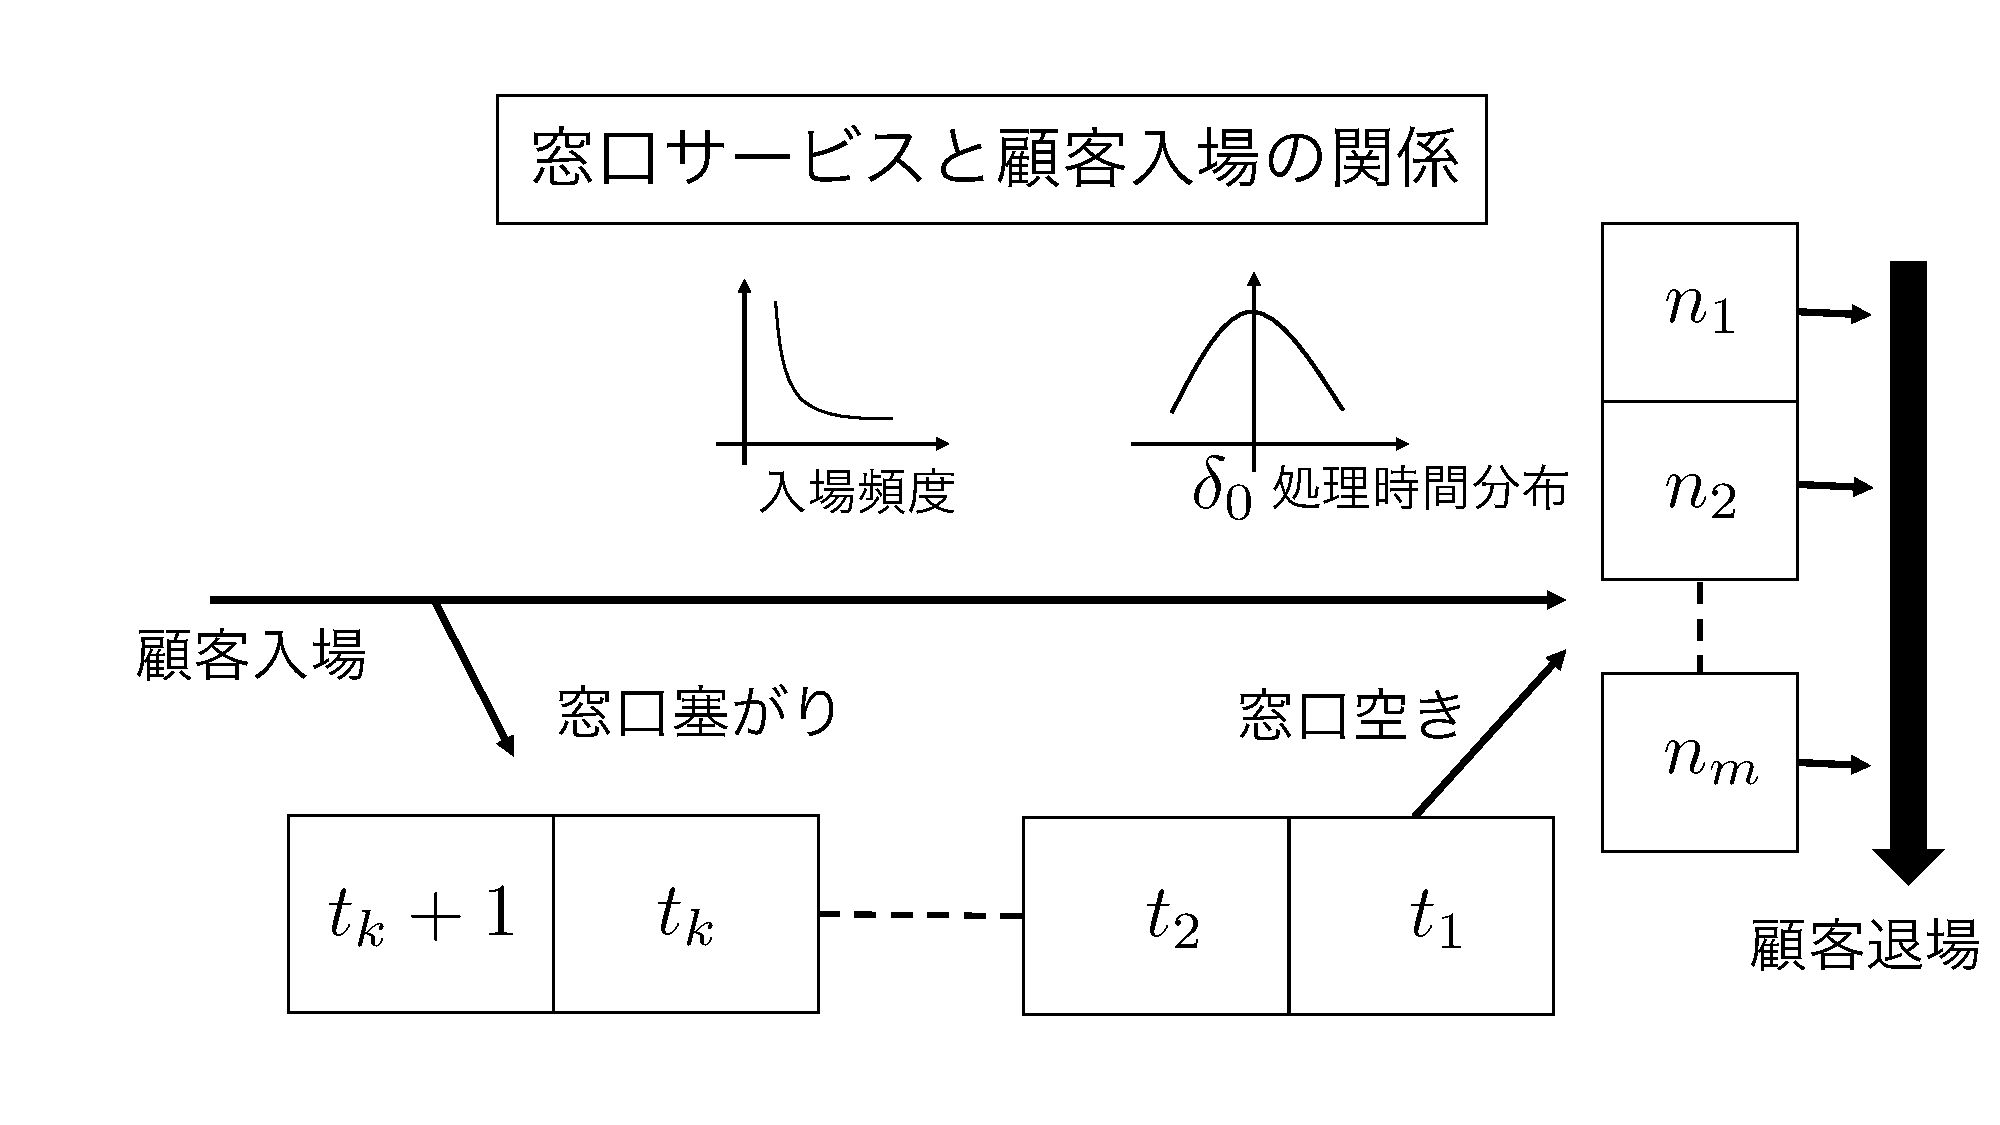
\includegraphics[height = 80mm  ] {figures/layout2.pdf}
\caption{窓口サービスと顧客入場の関係}
\label{fig:待ち行列概要}
\end{center}
\end{figure}

\clearpage

\subsection{モンテカルロ法}
モンテカルロ法とは,乱数を用いたシミュレーションを行うことにより近似解を求める計算方法である.この方法を使うことにより解析的に解くことができない問題でも,多くのシミュレーションを繰り返すことによって近似解を求めることができる.応用範囲が広く,問題によっては他の数値計算法より簡単に適用できるが,問題として高い精度を得ようとすれば計算回数が膨大になってしまうという欠点もある.例として,精度を1桁上げるためには試行回数Nを100倍にしなくてはならない.しかし,この欠点も近年ではコンピュータの計算能力の向上によって解消されつつある.

\subsection{安定状態}
安定状態とは,シミュレーションを行なった際,顧客の平均待ち時間が一定で安定している状態のことをいう.
この時の平均待ち時間は顧客1人1人の待ち時間を足していき顧客の数で割って求める.
また安定状態にある時の条件は,窓口での処理時間$x$,流れ密度$\alpha$,窓口の数$y$の関係が

(A)$x\alpha < y$

\noindent
が成り立つ時に安定状態となる.
\clearpage

\section{開発に使用した言語について}
\subsection{HTML}
HTMLとは「Hyper Text Markup Language(ハイパーテキスト・マークアップ・ランゲージ)」のことで,主にWebページを作成するための言語である\cite{html}.
現在のインターネットで公開されているWebページのほとんどは,HTMLで作成されている.ハイパーテキストに目印をつける言語と日本語に訳すことができる.

またHyper Text(ハイパーテキスト)とは,ハイパーリンクを埋め込むことができる高機能なテキストのことであり,文書中の文字や画像にWebサイトのURLを設定することが可能である.
そしてHTMLの特徴として,このハイパーリンク機能で関連する情報同士を結びつけて,情報を整理するということが挙げられる.
ハイパーリンクの概念図を図\ref{fig:hyper}に示す.
\begin{figure}[h]
\begin{center}
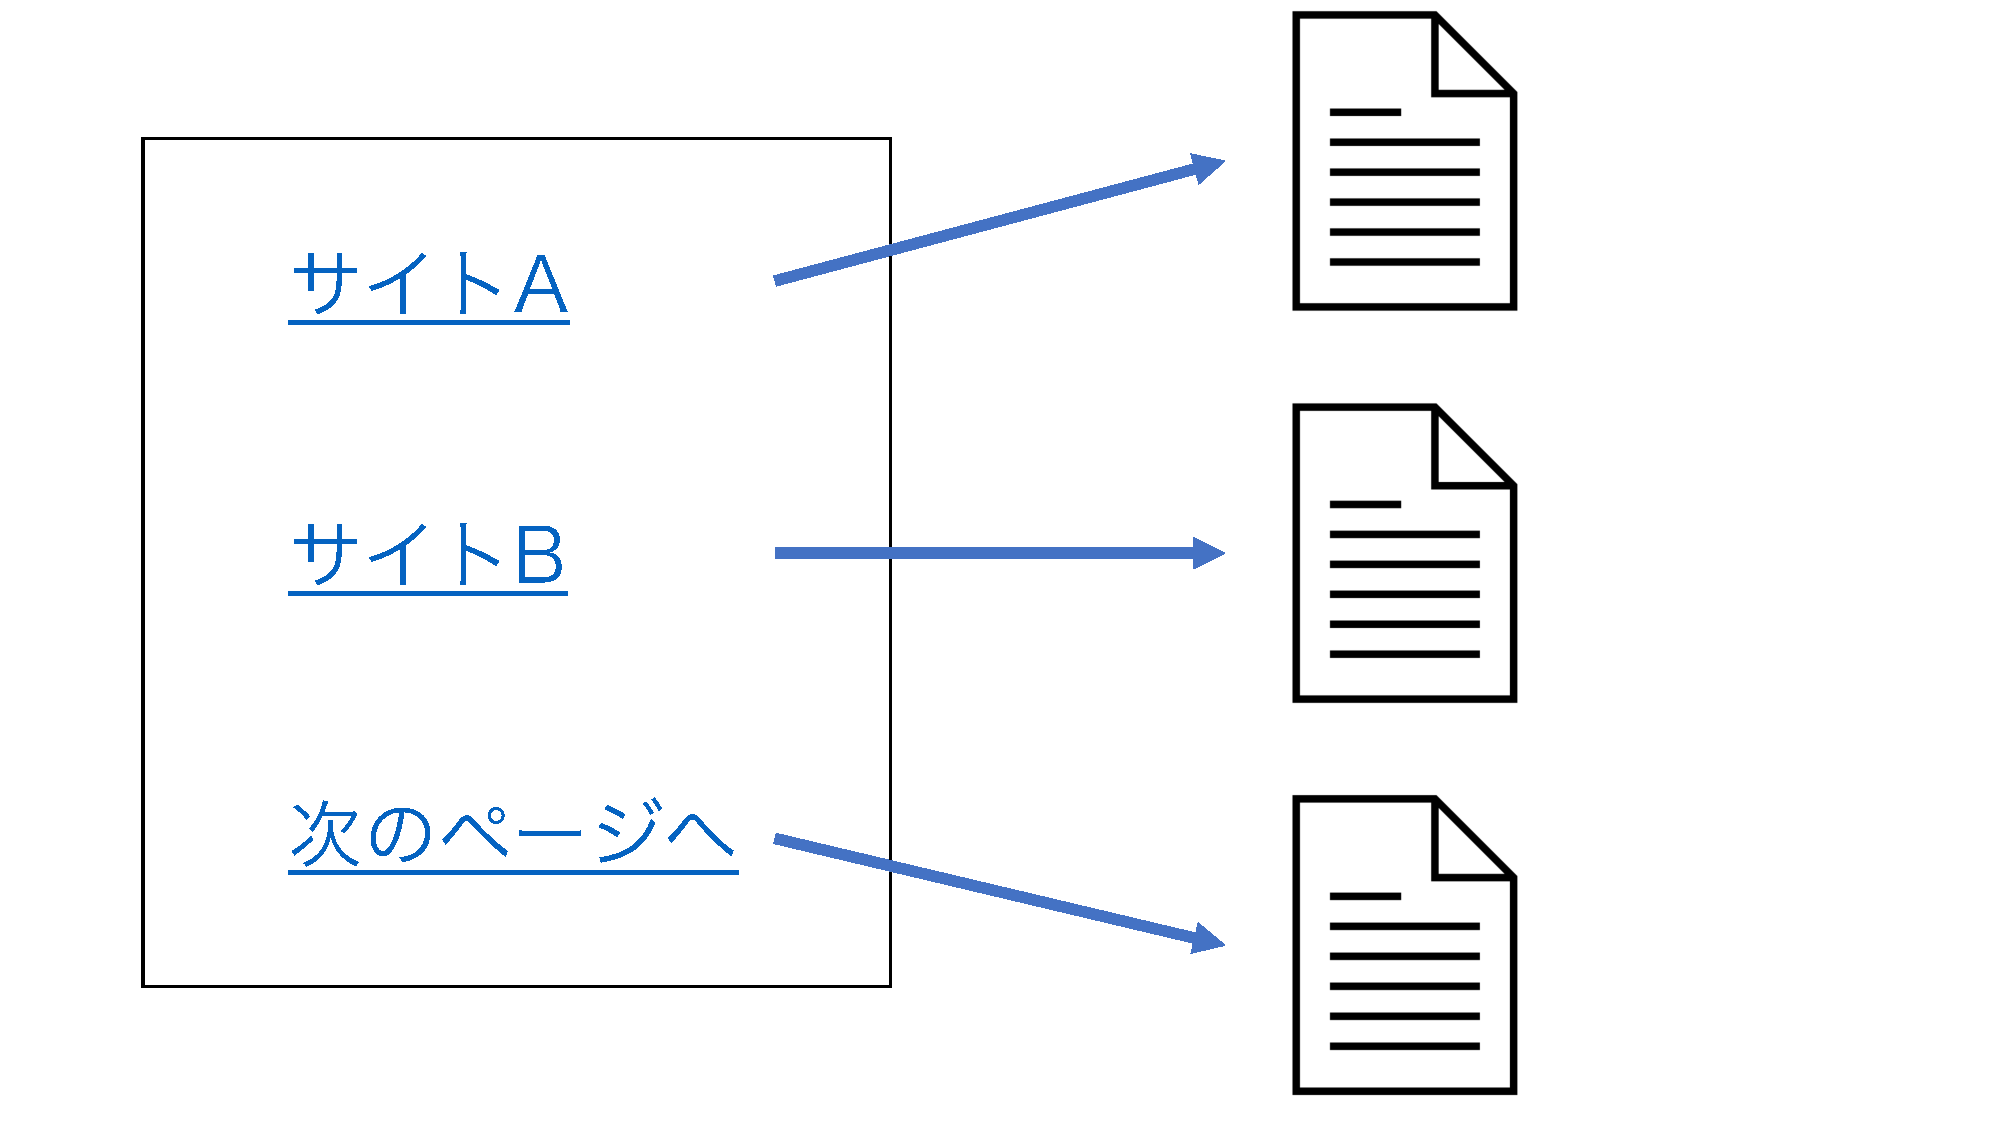
\includegraphics[width = 100mm ] {figures/hyperlink.pdf}
\caption{ハイパーリンクとは}
\label{fig:hyper}
\end{center}
\end{figure}


またもう1つの特徴として,見出し・段落・表などHTML文書内で各部分の役割が分かるように目印をつけることがある.これら各部分をelement(要素)と呼ぶ.
HTMLの要素について,図\ref{fig:html_elem}に示す.
\begin{figure}[h]
\begin{center}
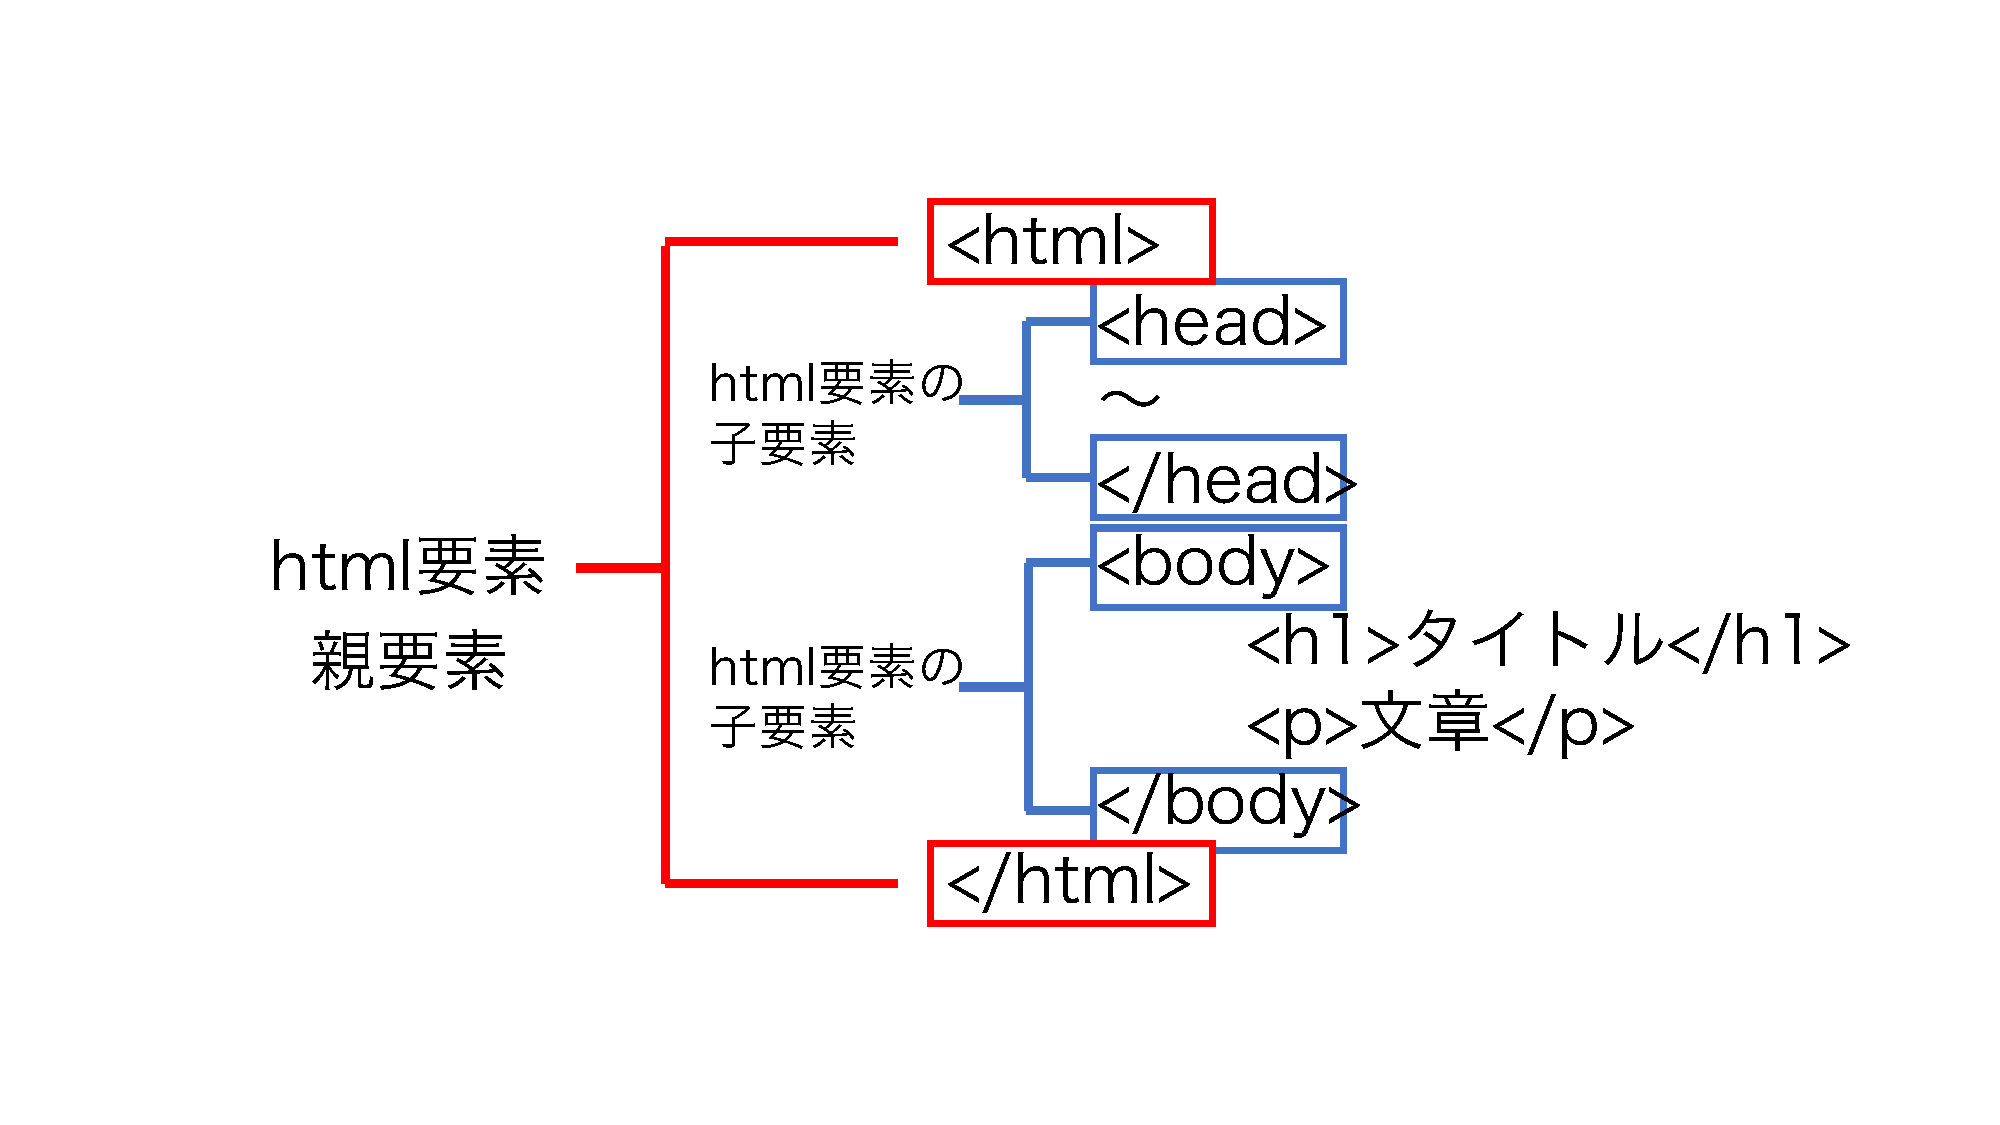
\includegraphics[height = 70mm ] {figures/html_ele.pdf}
\caption{HTMLの要素とは}
\label{fig:html_elem}
\end{center}
\end{figure}

\clearpage

そして,これらelementをHTML内に定義するための記号としてHTMLタグというものが存在する.代表的なものとして以下のものがある.
\begin{enumerate}[label=(\roman*)]
	\item <html></html>:HTML文書を定義,コード全体を囲む
	\item <body></body>:本文の設計を定義,WEBページに実際に表示される部分
	\item <a></a>:ハイパーリンクを定義
	\item <title</title>:タイトルを定義
\end{enumerate}

HTMLは基本的にこれらのタグを使用して要素を囲んでいくことで作成することができるため,プログラミング学習初心者にも分かりやすい言語とされている.
\clearpage

\subsection{CSS}
CSSとは「Cascading Style Sheets(カスケーディング・スタイル・シート)」のことであり,WEBページのスタイル・デザインを指定するための言語である\cite{css}.
基本的にHTMLと組み合わせて使用する.
HTMLで定義した見出しや文章の色や大きさ,要素の位置関係など細かく指定することができる.HTML単体でWebページを作成することができるが,CSSと組み合わせることで様々な変化をもたらすことができるので,CSSはWebページのデザイン性を高める上で有効である.

またCSSのスタイル定義の仕組みとして,「セレクタ」「プロパティ」「値」の3要素が存在する.
これらの要素はCSSの「どこの」,「何を」,「どうするのか」を指定している.
もう少し具体的に説明すると「セレクタ」はスタイル適用する場所を示し,「プロパティ」はどんな属性を変えるのかを示し,「値」では指定された場所にある属性を「どう」変えるのかを指定している.
実例として図\ref{fig:CSS_ex}に示す.

\begin{figure}[h]
\begin{center}
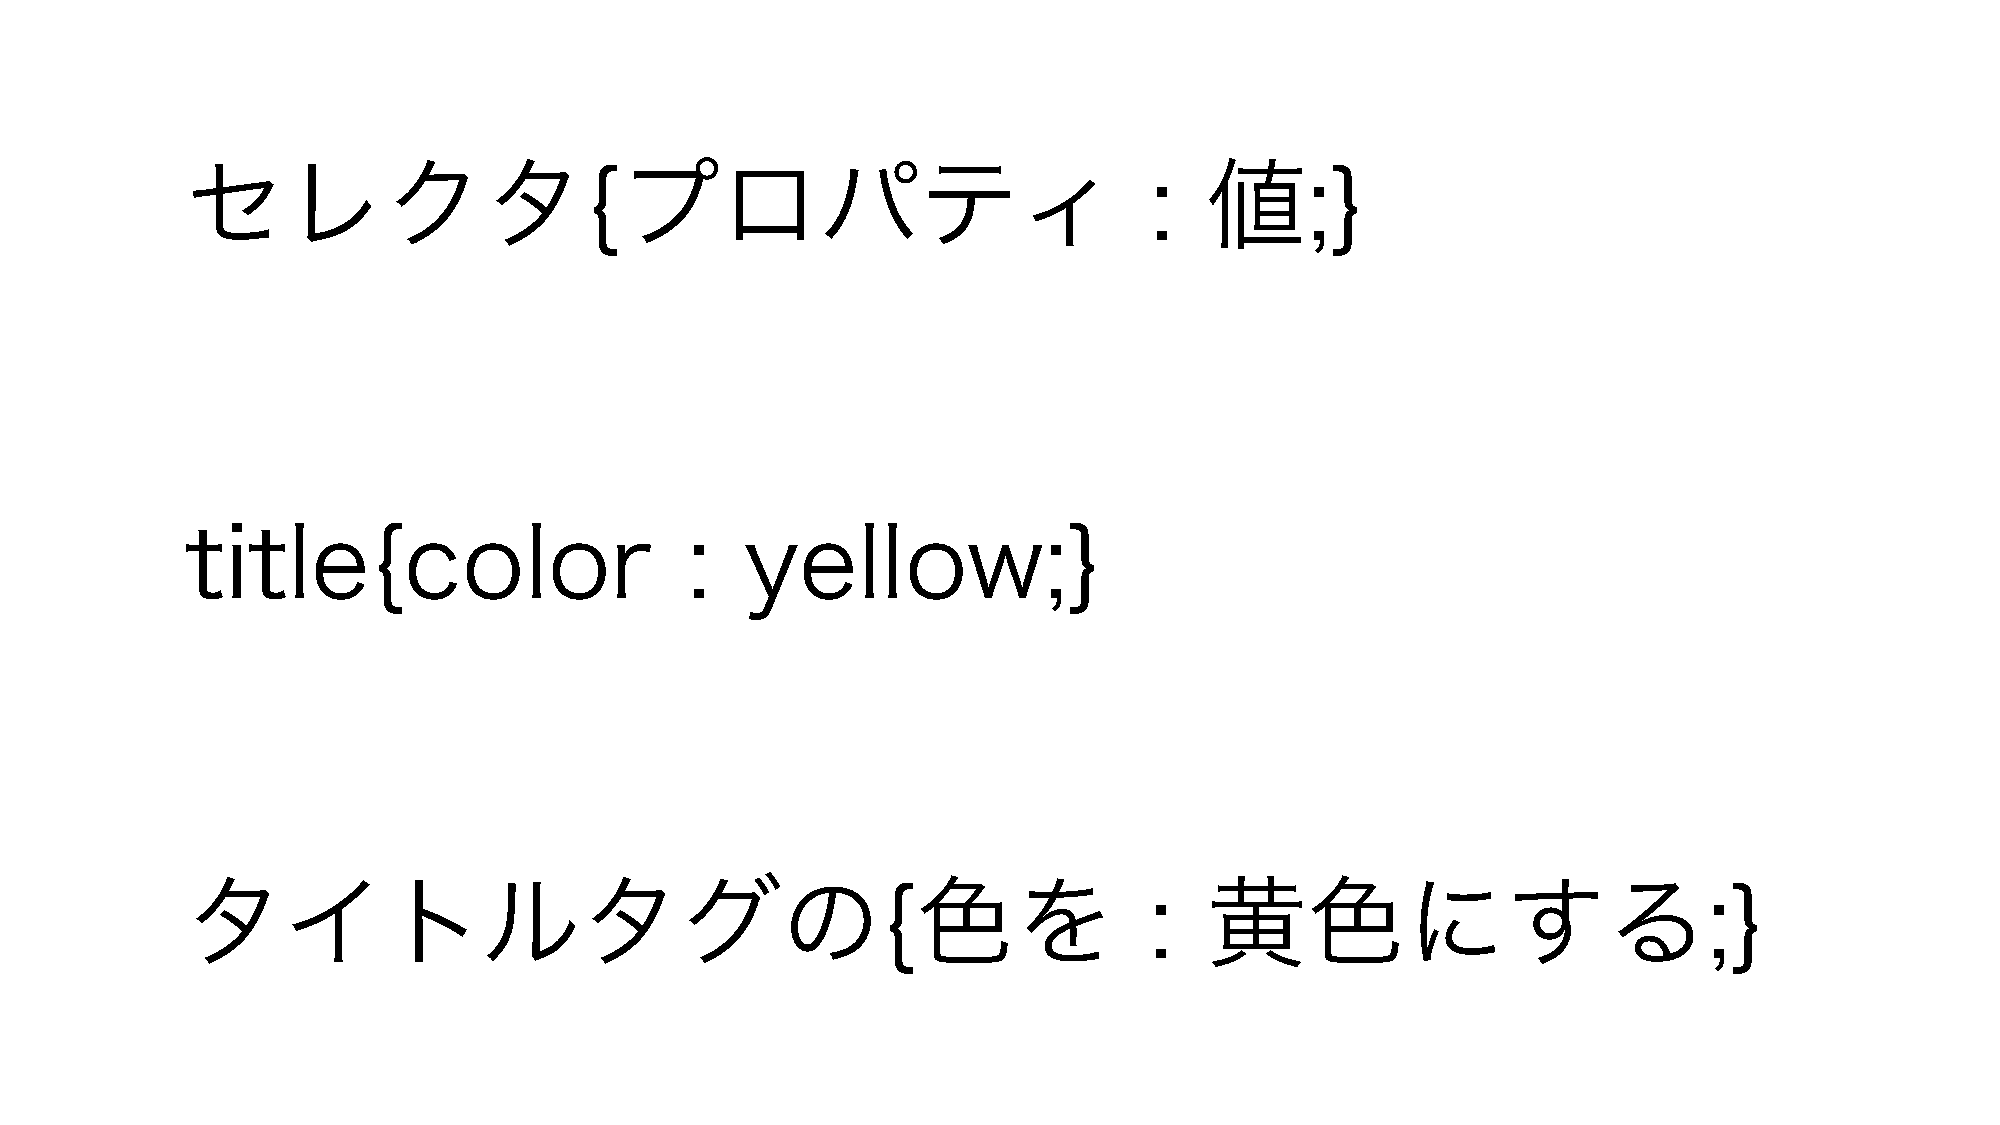
\includegraphics[height = 80mm ] {figures/css_ele.pdf}
\caption{CSSの使い方例}
\label{fig:CSS_ex}
\end{center}
\end{figure}

\clearpage

\subsubsection{CSSの必要性}
Webページを作成する上でHTMLだけで見栄えを制御することもできなくはない.
しかし,WebページのスタイリングにHTMLを用いるべきではない.
理由としてHTMLは情報構造を定義するための言語であり,スタイリングのような本来の役割とは違った使い方をするとコンピュータや検索エンジンに理解されないでたらめな文書構造になってしまうことがある.
ユーザーの検索エンジンによってうまくWebページが表示されなくなってしまう.
またCSSファイルとして独立させることで,HTML内にある関連箇所を逐一直さなくても,CSSファイルを変更するだけで一括で変更することが可能である.
つまりメンテナンスが行いやすくなるということも必要性として挙げられる\cite{css2}.

\clearpage

\subsection{JavaScript}
JavaScriptとはWebサイトやシステム開発に使われている言語である\cite{js}.
動的なWebページを作成するが得意でユーザーのアクションに応じたコンテンツの表示や,グラフィックアニメーションなども表示することができる.
HTMLとCSSで構築されたWebサイトに動きを加えたり,様々なWebサービスを実現できる.
つまり,HTMLとCSSに対して指示出しの役割を持つプログラミング言語である.

\subsubsection{Javaとの違い}
JavaScriptとJava,名前からして似ているプログラミング言語かと思う.
いくつかの共通点はあるが,全く別の言語である.
「JavaScript」は開発当初「LiveScript」と呼ばれていたが,その当時人気のあったプログラミング言語の「Java」にあやかって「JavaScript」という名前に変更された。
違いとして,「Java」はオブジェクト指向プログラミング言語であるのに対して,「JavaScript」はオブジェクト指向スクリプト言語である.
スプリクト言語とは,プログラミングの記述や実行が容易なプログラミング言語を指す.
また,「Java」はソースファイルをコンパイルし、実行ファイルを実行することでプログラムを走らせることが可能である。
一方で「JavaScript」のプログラムは単体で動作させることができない.
このようにJavaScriptとJavaは名前は似ているが,この2つの言語は性質が異なるプログラミング言語である.
\clearpage

\section{開発したシミュレータについて}
\subsection{教材に必要な機能} 
\begin{figure}[h]
\begin{center}
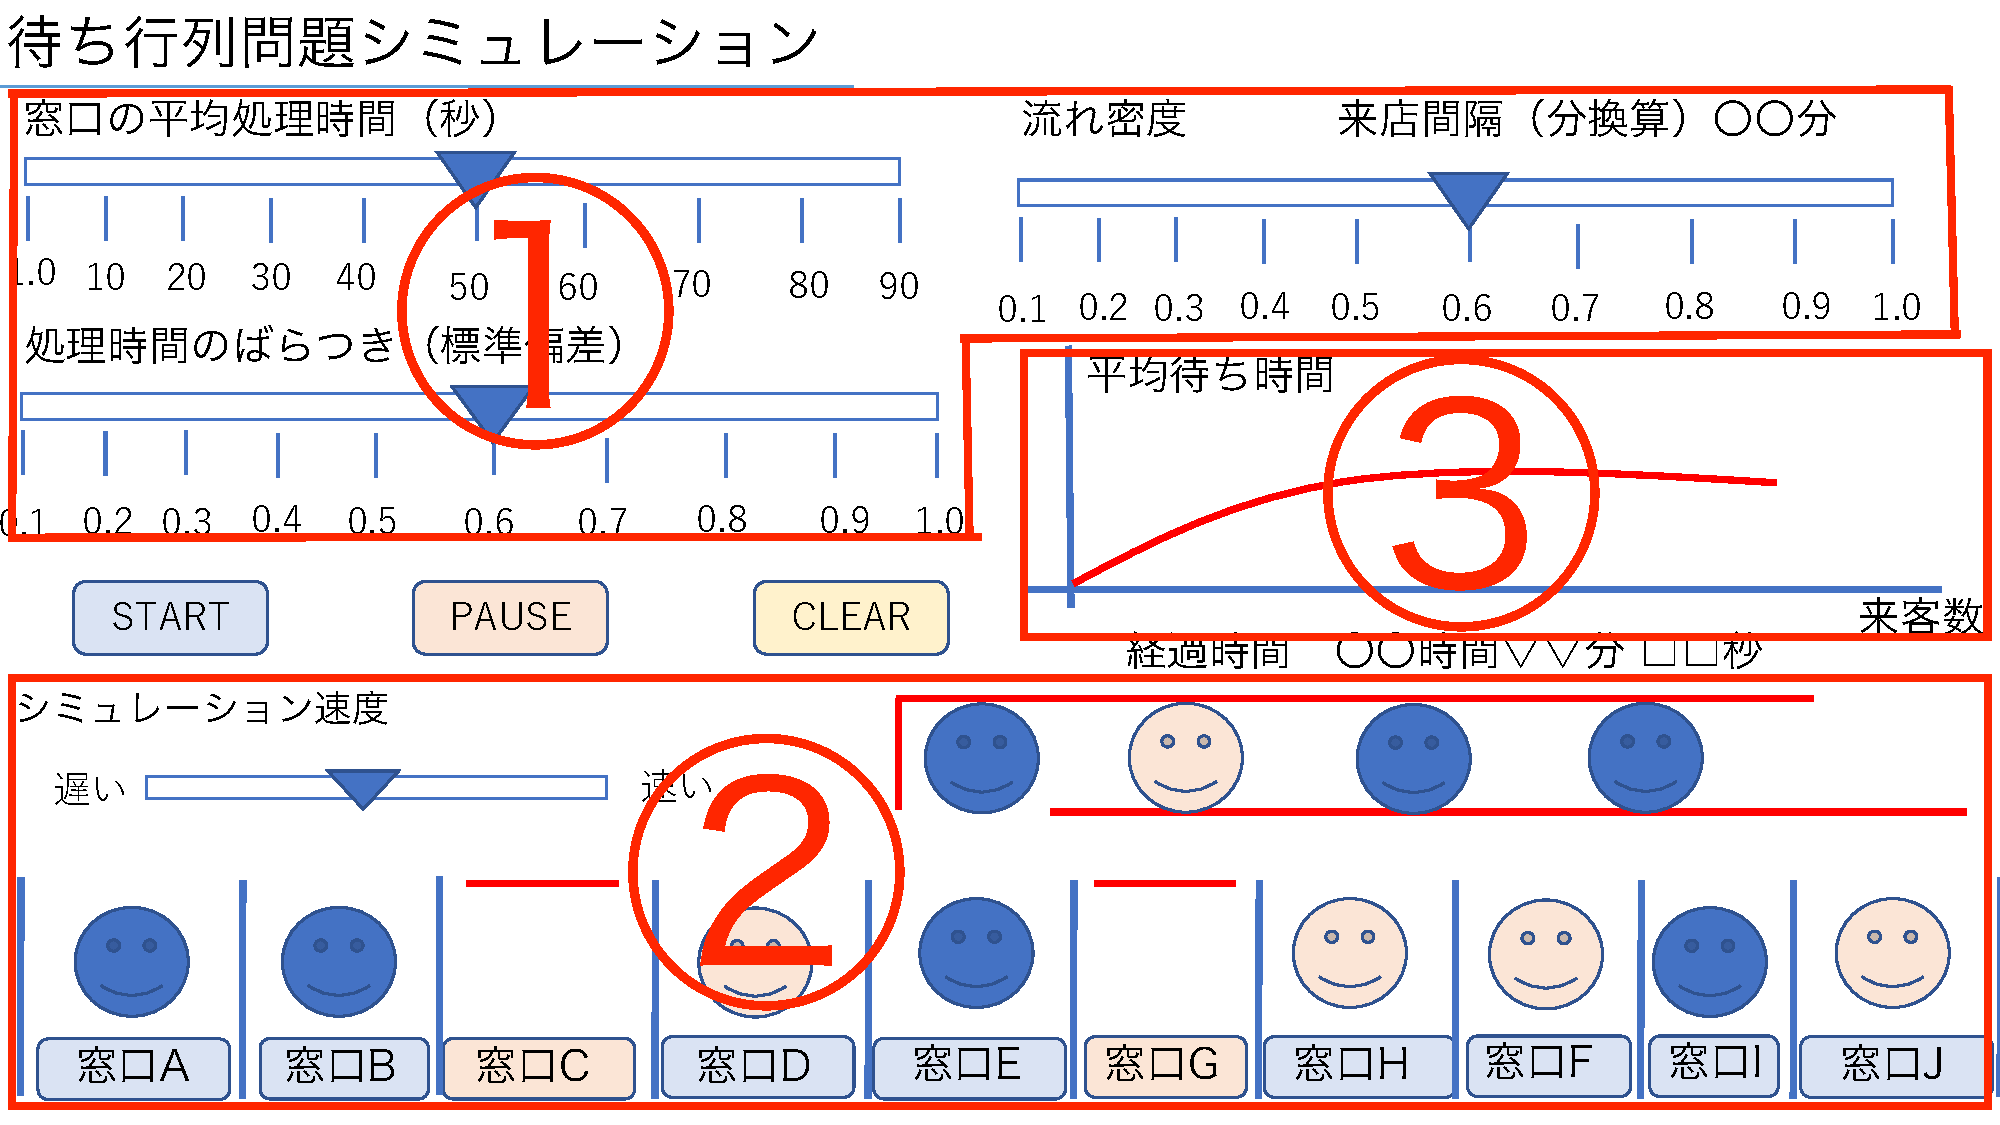
\includegraphics[height = 80mm ]{figures/simulator_layout.pdf}
\caption{待ち行列問題シミュレータ教材のレイアウト}
\label{fig:layout}
\end{center}
\end{figure}
この章では,待ち行列問題シミュレータ教材を開発する上で,学習者の理解度向上を考えどのような機能があるか説明していく.
図\ref{fig:layout}は開発する以前に作成した待ち行列問題シミュレータ教材のレイアウトである.

\vskip\baselineskip
<待ち行列状態の表示>

本研究はアニメーションをより現実的な動きに寄せブラウザ上への移植及び改良することでより利用者の理解度の向上を目的としている.
そのため今回開発する教材は過去の研究で作成されたものを使用した.
基本的なUIはそのままに,アニメーション部の改良が本研究の大きな目標である.
そうすることで,より現実に近い動きになりさらに理解度の向上が見込めると考えた.

\vskip\baselineskip
<待ち行列状態を設定するパラメータの設定>

待ち行列の状態は,様々なパラメータの影響を受け変化する.
そのパラメータとして,窓口の数,客の流れ密度,サービスに必要な平均時間,処理時間のばらつき(標準偏差)がある.
これらパラメータを変化させた時,待ち行列の状態にどのような変化が起きるか,学習者に視覚的に理解させる必要がある.
そのため,学習者がパラメータを設定できるようにした.

\vskip\baselineskip
<アニメーションの再生・一時停止・初期化>

アニメーションを行うことで,現象を視覚的に体験でき学習者の理解を促すことが可能である.
今回作成予定の教材では,過去の研究で作成されたものと同様にアニメーションをスタートさせるSTARTボタン,アニメーションを一時停止させるPAUSEボタン,動作の画面やパラメータを初期化するClearボタンを作成した.
\clearpage
\vskip\baselineskip

<窓口での処理と窓口ボタン>

窓口での処理は,平均待ち時間の安定状態を求めるために実際の窓口での現象を再現する必要がある.
そのためには開いている窓口の数が重要となる.
設定したパラメータの適した窓口数を求めるために実行中に変更できる窓口の開閉ボタンを作成した.

\vskip\baselineskip

<平均待ち時間のグラフ化>

設定したパラメータに基づいた,計算の結果をグラフ化し変化の状態を可視化した.
可視化することによって,平均待ち時間の安定状態・状態遷移が理解しやすくなると考えた.

\clearpage

\subsection{開発した教材の実行例}
前述であげた機能について,実行例をあげていく.
図\ref{fig:layout_ex}は開発した待ち行列問題教材の画面である.
\begin{figure}[h]
\begin{center}
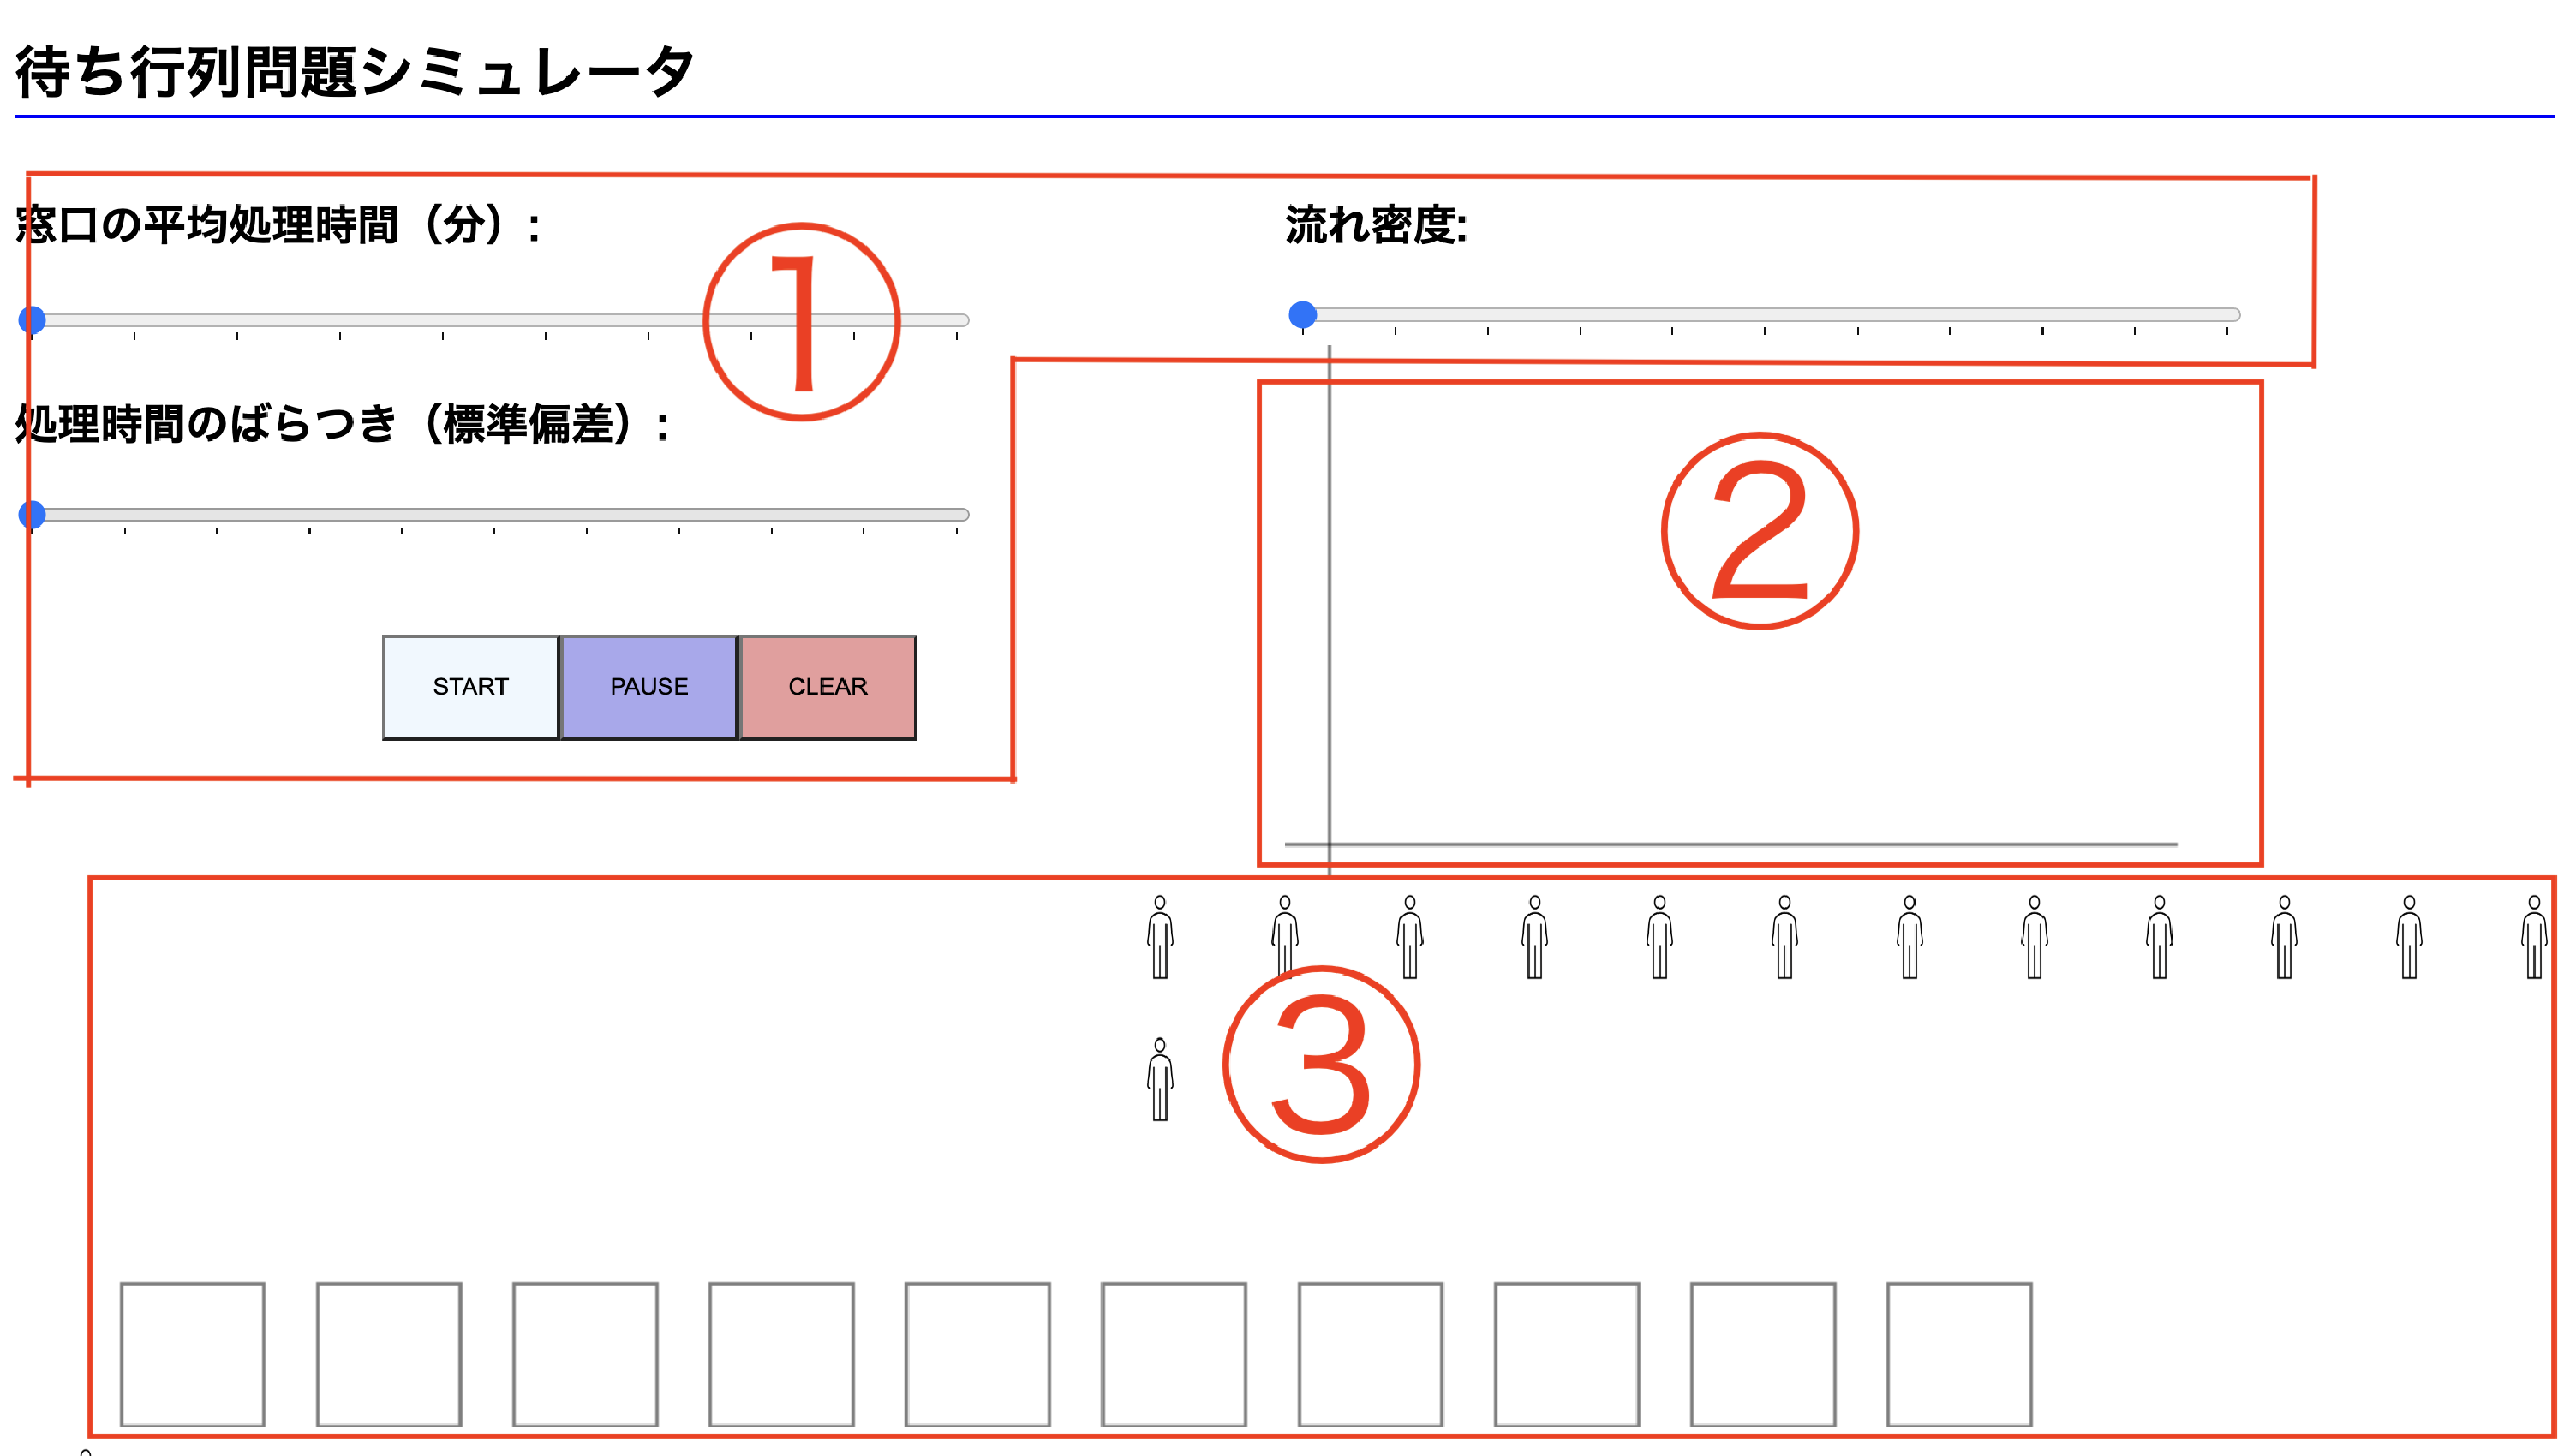
\includegraphics[height = 80mm ] {figures/layout_ex.pdf}
\caption{開発した待ち行列問題シミュレータ教材のレイアウト}
\label{fig:layout_ex}
\end{center}
\end{figure}

①は窓口の平均処理時間,客の流れ密度,処理時間のばらつき(標準偏差)をそれぞれ変更できるスライダーがある.
また,処理時間のばらつき(標準偏差)の下にある3つのボタンは左から,STARTボタン,PAUSEボタン,CLEARボタンである.

②は教材を実行した際に,平均待ち時間の値を表示するグラフの領域である.

③では,設定したパラメータに応じたアニメーションを表示する.③下部にある四角形は窓口を表しており,窓口の数を増減させたい場合は,各四角形をクリックすることで窓口を開閉できる.

\clearpage

\subsubsection{各パラメータについて}
待ち行列の状態は,窓口数,窓口の平均処理時間,客の流れ密度,処理時間のばらつき(標準偏差)のパラメータが影響している.
これらのパラメータのうち,窓口の平均処理時間,客の流れ密度,処理時間のばらつき(標準偏差)の値は図\ref{fig:layout_ex}①部分のスライダーで設定する.
窓口の平均処理時間は0〜10,流れ密度は0〜1.0,処理時間のばらつきは0〜1.0の値を設定できるようになっている.

\begin{figure}[h]
\begin{center}
\includegraphics[height = 80mm ] {figures/lay.pdf}
\caption{設定するパラメータ}
\label{fig:layout_ex}
\end{center}
\end{figure}

\clearpage

\subsubsection{実行方法について}
実行方法について図\ref{fig:設定}に示す.
前述した図\ref{fig:layout_ex}の各パラメータを設定し,STARTボタンを押すことでアニメーションが開始する.
図\ref{fig:アニメ実行}は,窓口数:10,窓口の平均処理時間:6,客の流れ密度:0.8,処理時間のばらつき:0.1に設定した画面である.
図\ref{fig:アニメ実行}は,実際にパラメータを設定し実行した際の画面を示している.
\begin{figure}[h]
\begin{center}
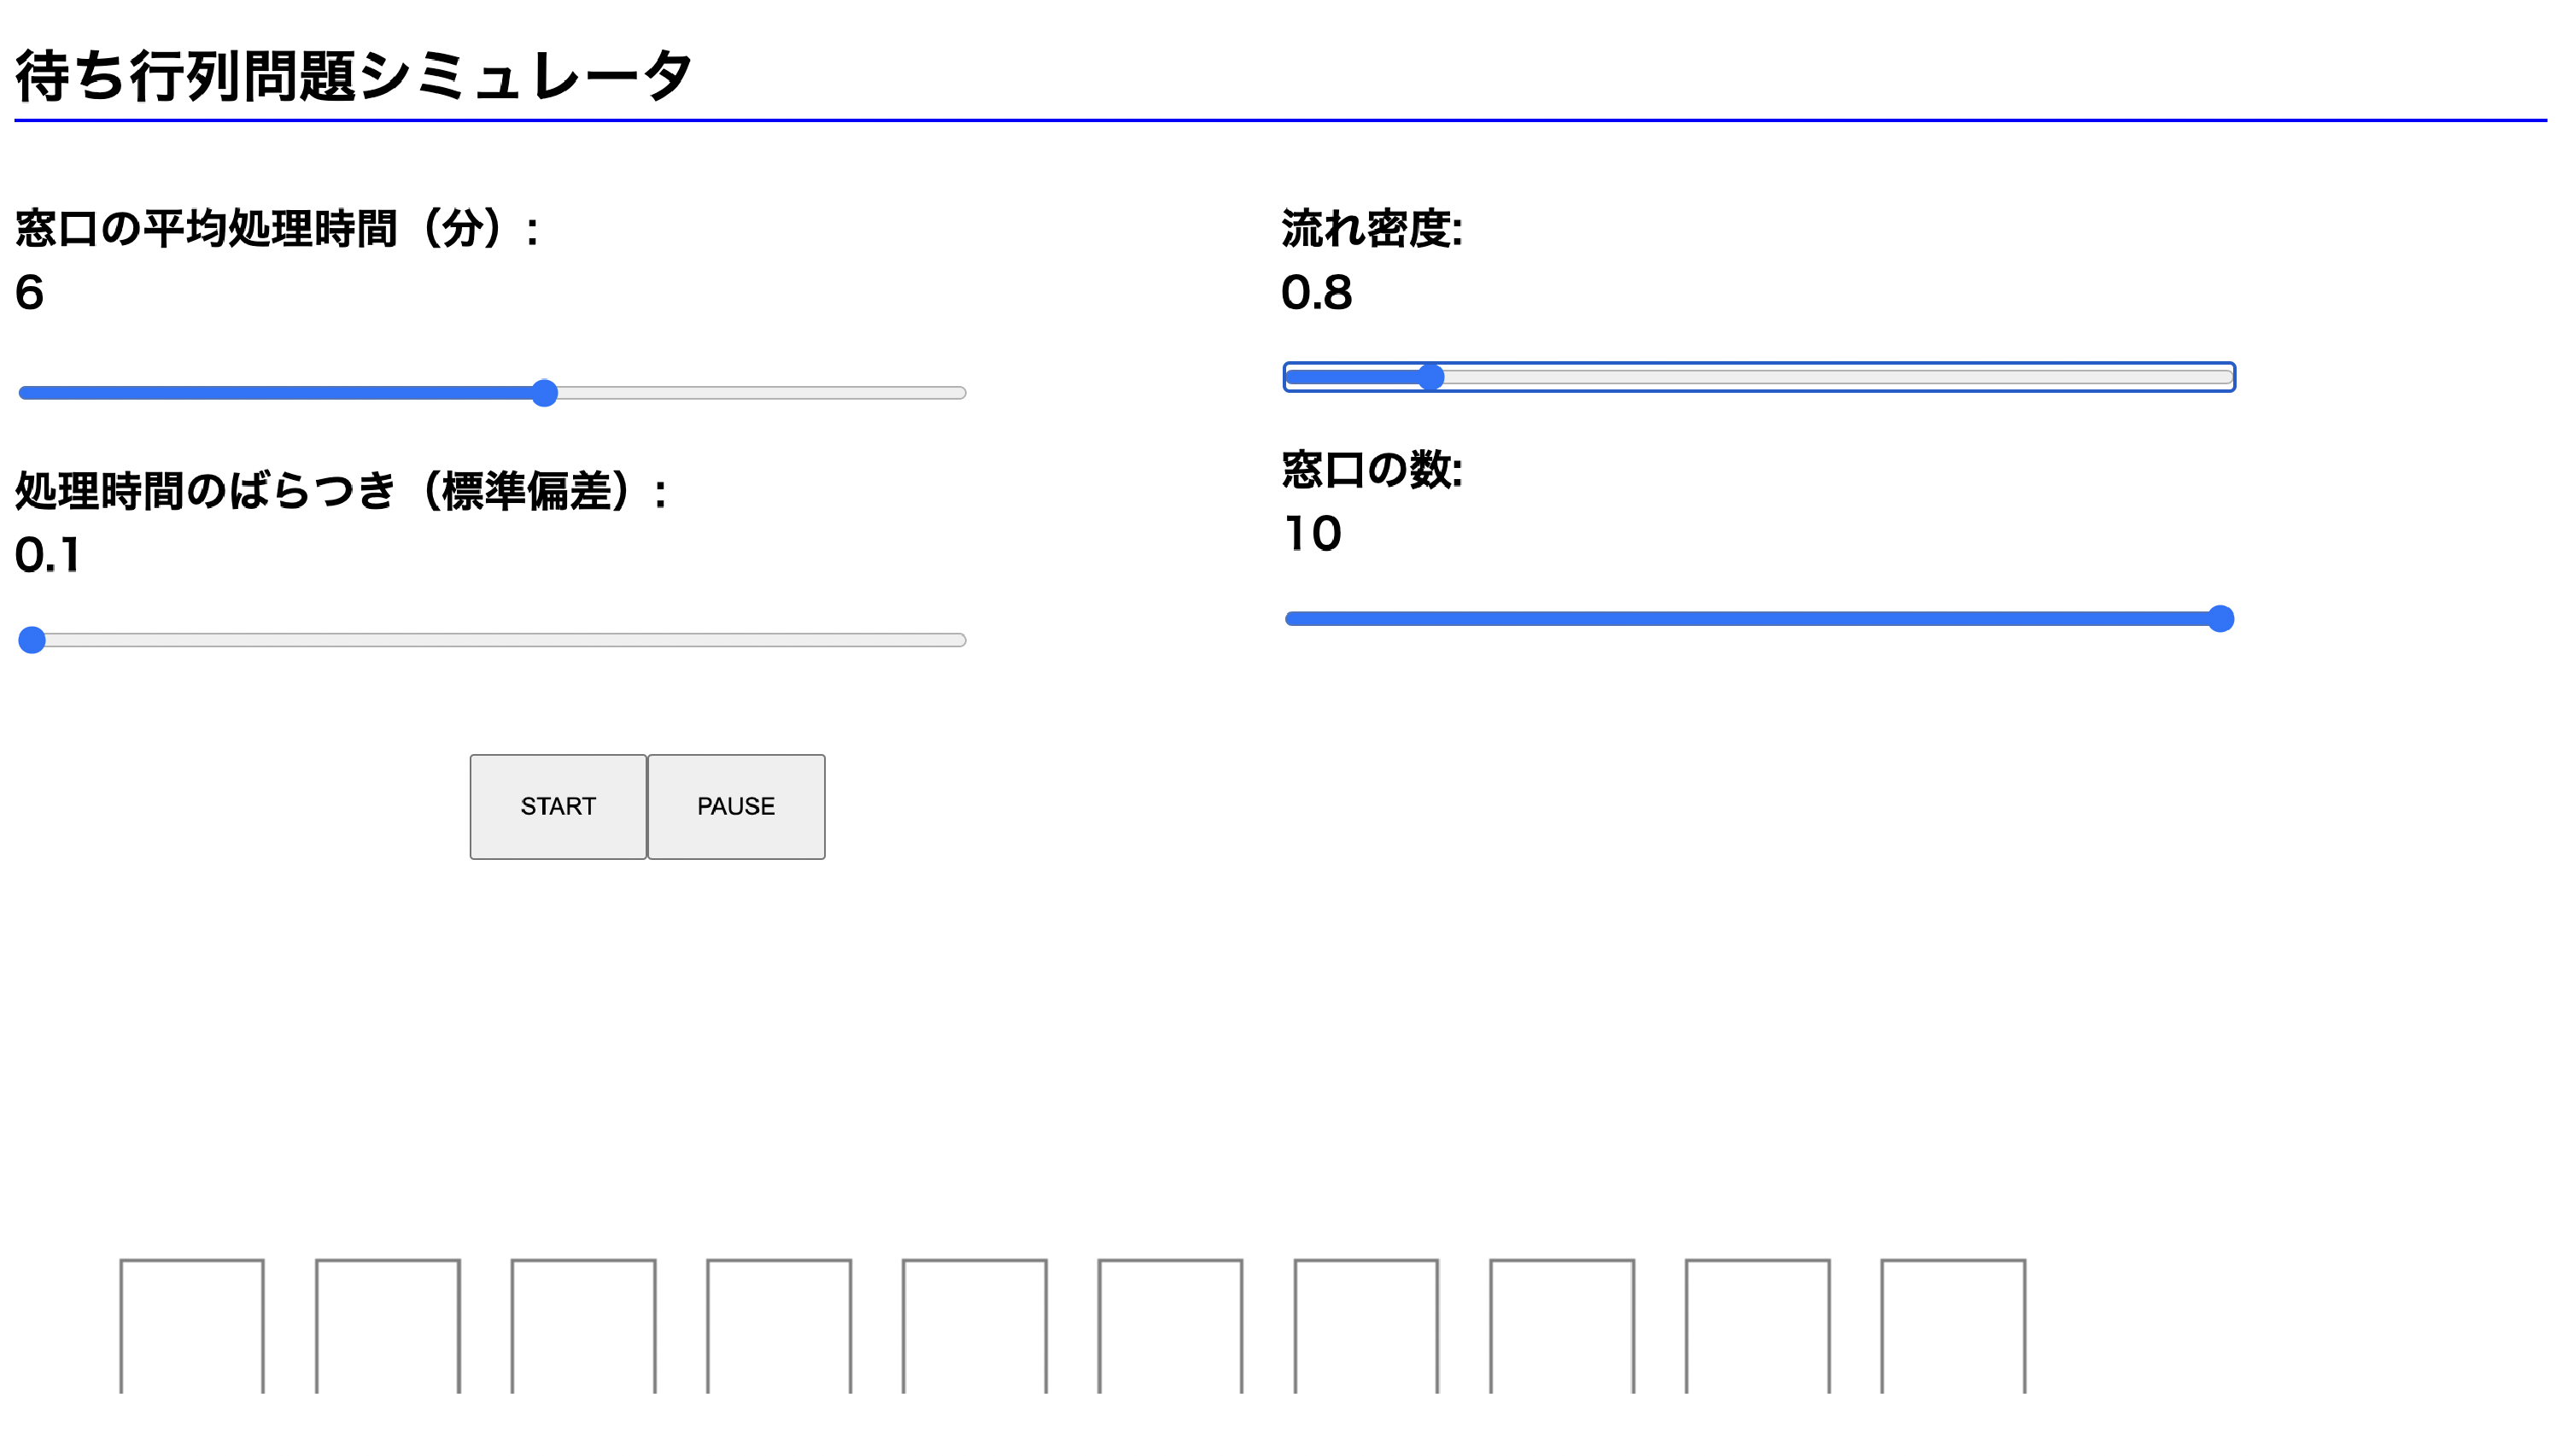
\includegraphics[height = 80mm ] {figures/lay_para.pdf}
\caption{パラメータ設定後の画面}
\label{fig:設定}
\end{center}
\end{figure}

\begin{figure}[h]
\begin{center}

\includegraphics[height = 80mm ] {figures/figure_sample.pdf}
\caption{アニメーション実行例}
\label{fig:アニメ実行}
\end{center}
\end{figure}

\clearpage


\section{おわりに}
本研究では,先行研究をもとに視覚的・直感的に理解できることを目的とした待ち行列問題シミュレータをブラウザへ改良を行い,移植することを目的とした.

問題点として,先行研究は開発環境が古く現在は使用できないこと,アニメーションが画像を切り替えていくことによる擬似的なアニメーションであり,なめらかなアニメーションではなかったという点がある.

結果として,先行研究と比較してアニメーションの部分を改良することができた.
具体的には画像を切り替えていくことによる擬似的なアニメーションではなく,人の画像を座標を指定して実際に窓口の前まで動かし,窓口から退場の動きも付け加えることができた.

本教材が科目「数値計算」における「待ち行列問題」を理解する上で少しでも役に立てれば嬉しい.

\clearpage

\section{謝辞}
本研究の遂行及び本論文作成にあたり,多大なるご指導,ご助言を頂きました  須田 宇宙准教授に深く感謝の意を表します.
\clearpage

\begin{thebibliography}{99}
\bibitem{sotuken16}平成16年度 卒業論文 モンテカルロ法による待ち行列問題のマルチメディア教材  (薄井英彦・梅山卓也)
\bibitem{soumu} 総務省統計局 最適な設備投資を把握”, \url{https://www.stat.go.jp/naruhodo/15_episode/toukeigaku/setubitoshi.html}, 2022/12/5参照
\bibitem{html} HTMLクイックリファレンス”, \url{http://www.htmq.com/}, 2022/12/5参照
\bibitem{css}HTML・CSSのそれぞれの基礎知識と違いとは? ”, \url{https://www.sedesign.co.jp/blog/html-css}, 2022/12/6参照
\bibitem{css2}Web制作に欠かせないCSSとは?役割や活用メリット、使い方などを解説します! ”, \url{https://persol-tech-s.co.jp/hatalabo/it_engineer/502.html}, 2022/12/6参照
\bibitem{js}JavaScriptとは? modis ”, \url{https://www.modis.co.jp/candidate/insight/column_29}, 2022/12/6参照
\bibitem{Exponential} 指数分布の意味と具体例 \url{https://manabitimes.jp/math/1006}
\end{thebibliography}

\end{document}